\documentclass[a4paper, oneside]{book}

\usepackage{geometry,url,graphicx, hyperref,subfig,enumitem, amsmath,float}
\usepackage{amsmath, amssymb, amsthm, mathtools, color, setspace}
\usepackage{fancyhdr, braket, etoolbox,booktabs,multirow}
\usepackage{xfrac, lmodern} % xfrac gives font errors, add lmodern to remove them. Check whether this remains a problem!
%\usepackage{hyperref}
%\usepackage[utf8]{inputenc}
%\usepackage{colorprofiles}
\usepackage[T1]{fontenc}

\begin{document}
	\begin{titlepage}
		%%%% LOGO %%%%
		\begin{figure}
			
\includegraphics[width=\linewidth]{tesi_images/logo.jpg}
		\end{figure}
		\center
		\textsc{\large Corso di laurea in Fisica}\\[0.2cm]
		\textsc{\normalsize Tesi di laurea triennale}\\[2cm]
		%\rule{\linewidth}{0.3mm} \\[1.2cm]
		
		% TITLE
		\begin{doublespace}
			\textbf{\LARGE A machine learning approach to the electrons and photons classification with the ATLAS detector at the LHC}
			\\[2cm]
		\end{doublespace}
		
		% AUTHOR
		\begin{minipage}{0.4\textwidth}
			\begin{flushleft}
				\emph{Autore:} \\[0mm]
				\textbf{Pietro Daniele} \\[4mm]
				\emph{Matricola:}\\
				906962 \\[4mm]
				\emph{Codice P.A.C.S.:}\\[0mm]
				07.05.-t
			\end{flushleft}
		\end{minipage}
		%
		\begin{minipage}{0.4\textwidth}
			\begin{flushright} 
				\emph{Relatore:} \\
				\textbf{Prof. Leonardo Carlo Carminati} \\[1.2em]
				\emph{Corelatori:} \\
				\textbf{Dott. Ruggero Turra} \\
				\textbf{Dott. Davide Mungo} \\[1.2em]
			\end{flushright}
		\end{minipage}\\[2cm]
		\vfill
		Anno accademico 2019-2020
		
	\end{titlepage}

\tableofcontents

	\chapter{LHC and the ATLAS detector}
		\section{The LHC}
			The CERN Large Hadron Collider (LHC) \cite{LHC design} is a two-ring, superconducting protons and heavy ions accelerator and collider installed in the 27 km-long LEP tunnel. It provides pp collisions at an unprecedent center of mass energy $\sqrt{s} = 13$ TeV.
			
			Inside the accelerator, two high-energy particle beams travel close to the speed of light before they are made to collide. The beams travel in opposite directions in separate beam pipes (two tubes kept at ultrahigh vacuum). They are guided around the accelerator ring by strong magnetic fields maintained by superconducting electromagnets\cite{LHC introduction},\cite{LHC site}.
				\subsection{LHC Layout}
					\begin{figure}[H]
						\centering
						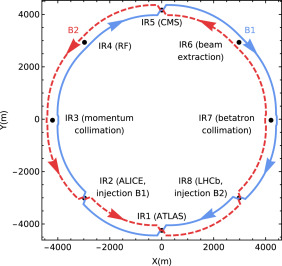
\includegraphics[width=0.3\textheight]{tesi_images/LHC_structure.jpg}
						\caption{LHC structure}
						\label{fig:LHC structure}
					\end{figure}
					The basic layout of the LHC follows the LEP tunnel geometry, as shown in Figure \ref{fig:LHC structure}. The LHC has eight arcs and eight straight sections. Each straight section is approximately 528 m long and can serve as an experimental or utility insertion. The two high luminosity experimental insertions are located at diametrically opposite straight sections: the ATLAS experiment is located at point 1 (IR1) and the CMS experiment at point 5 (IR5).
					
					Two more experimental insertions are located at point 2 and point 8 which also contain the injection systems for Beam
					1 and Beam 2, respectively. The injection kick occurs in the vertical plane with the two beams arriving at the LHC from below the LHC reference plane. The beams only cross from one magnet bore to the other at
					these four locations.
					
					The remaining four straight sections do not have beam crossings. Insertion 3 and 7 each contain two collimation systems. Insertion 4 contains two RF systems: one independent system for each LHC
					beam. The straight section at point 6 contains the beam dump insertion where the two beams are vertically
					extracted from the machine using a combination of horizontally deflecting fast-pulsed ('kicker') magnets and
					vertically-deflecting double steel septum magnets. Each beam features an independent abort system. \cite{LHC design} \\
					The protons travel inside along th LHC ring in opposite direction. The LHC beams are controlled by superconducting magnets, which have a working temperature of 1.9 K. There are two kinds of superconducting magnets (Figure \ref{fig:magnets}):
					\begin{itemize}
						\item the superconducting dipole magnets, which thanks to a 8.33 T magnetic field drive protons along the ring (circular orbit);
						\item superconducting quadrupole magnets, which keep the beams focused.
					\end{itemize} 
					\begin{figure}
						\centering
						\subfloat[][\emph{LHC dipole}]{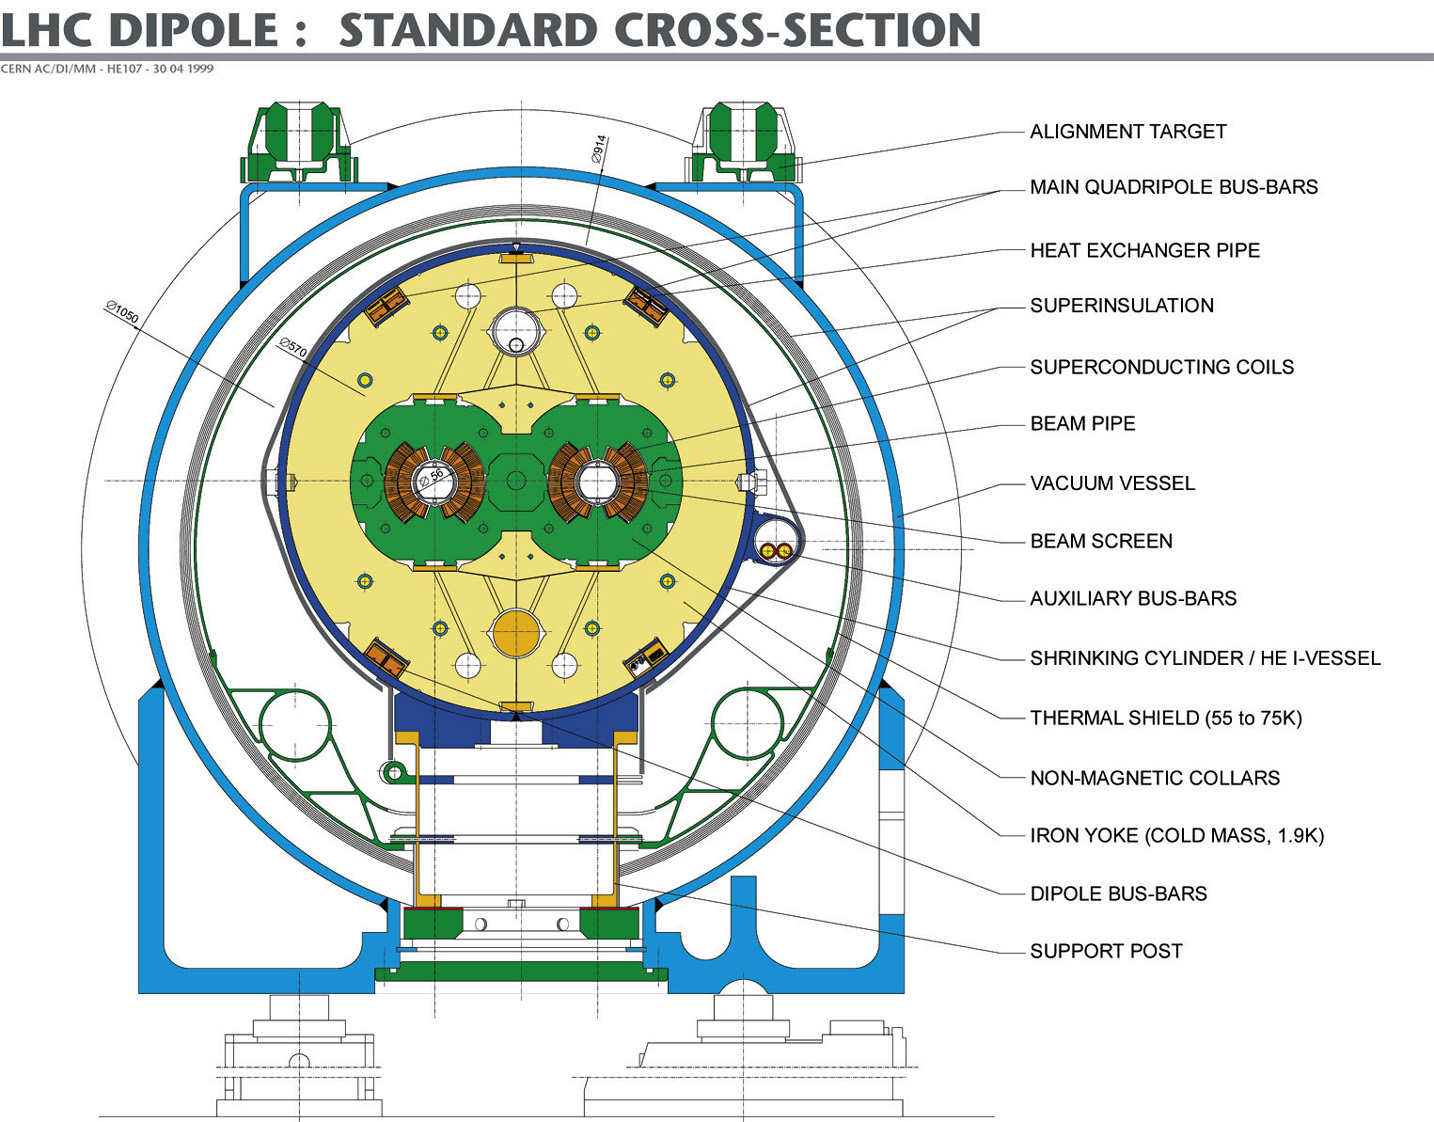
\includegraphics[width=.45\textwidth]{tesi_images/m_dipole.jpeg}} \quad
						\subfloat[][\emph{LHC quadpole}]{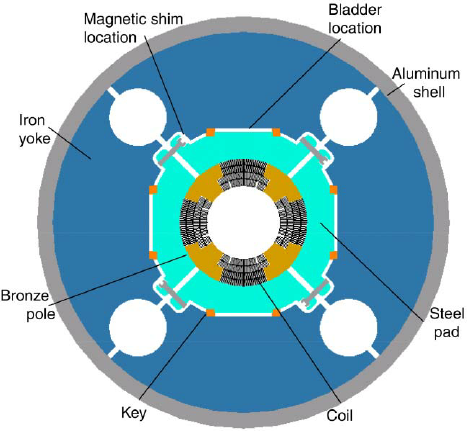
\includegraphics[width=.3\textwidth]{tesi_images/m_quad.png}} 
						\caption{LHC's superconducting magnets}
						\label{fig:magnets}
					\end{figure}
				\subsection{The CERN accelerator complex}
					Before being insert into LHC ring, particle beam is accelereted by the CERN accelerator complex \cite{Acc. complex}. It is a succession of machines which accelerate particles at increasingly higher energies. Each machine injects the beam into the next one, which takes over to bring the beam to an even higher energy, and so on. In  the  LHC, the  last  element  of  this  chain, each particle beam is accelerated up to the record energy of 6.5 TeV. At the CERN complex, protons are obtained by stripping electrons from hydrogen atoms, which are taken from a bottle containing hydrogen. Then protons are injected into the PS Booster (PSB) at an  energy of 50 MeV from Linac2. The  booster  accelerates  them  to  1.4  GeV.  The  beam  is  then  fed  to  the  Proton  Synchrotron  (PS)  where  it  is  accelerated  to  25 GeV. Protons are then sent to the Super Proton Synchrotron (SPS) where they are accelerated to 450 GeV. They  are  finally  transferred  to  the  LHC  (both  in  a  clockwise  and an anticlockwise direction) where they are accelerated for 20 minutes to 6.5 TeV. Beams circulate for many hours inside the LHC beam pipes under normal operating conditions.
					In addition to accelerating protons, the accelerator complex can also accelerate lead ions. 
					\begin{figure}
						\centering
						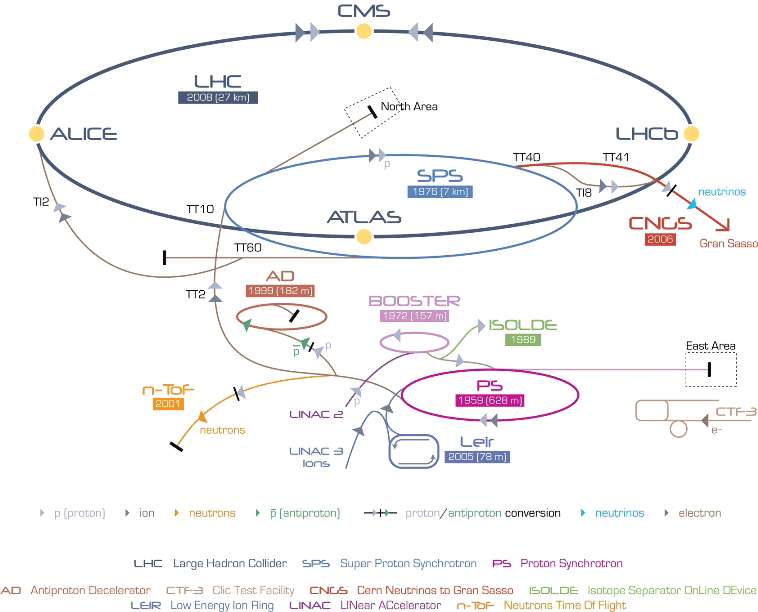
\includegraphics[width=0.45\textheight]{tesi_images/CERN.png}
						\caption{LHC and CERN's complex accelerator}
						\label{fig:CERN structure}
					\end{figure}
				\subsection{Proton-proton collisions}
					The number of events per second generated in the LHC collisions is given by:
					$$
					N_{i} = L\sigma_{i}
					$$
					where $\sigma_{i}$ is the cross section for the process under study and $L$ the instantaneous machine luminosity. $L$ depends only on the beam parameters and can be written for a Gaussian beam distribution as: 
					$$
					L = \frac{N_b^2n_bf_{rev}\gamma_r}{4\pi\epsilon_n\beta^*}F
					$$
					where $N_b$ is the number of particles per bunch, $n_b$ the number of bunches per beam, $f_{rev}$ the revolution frequency, $\gamma_r$ the relativistic gamma factor, $\epsilon_n$ the normalized transverse beam emittance, $\beta^*$ the beta function at the collision point and $F$ the geometric luminosity reduction factor due to the crossing angle at the IP. The luminosity had various values during ATLAS activity as shown in the Figure \ref{fig:lum}.
					
					\begin{figure}
						\centering
						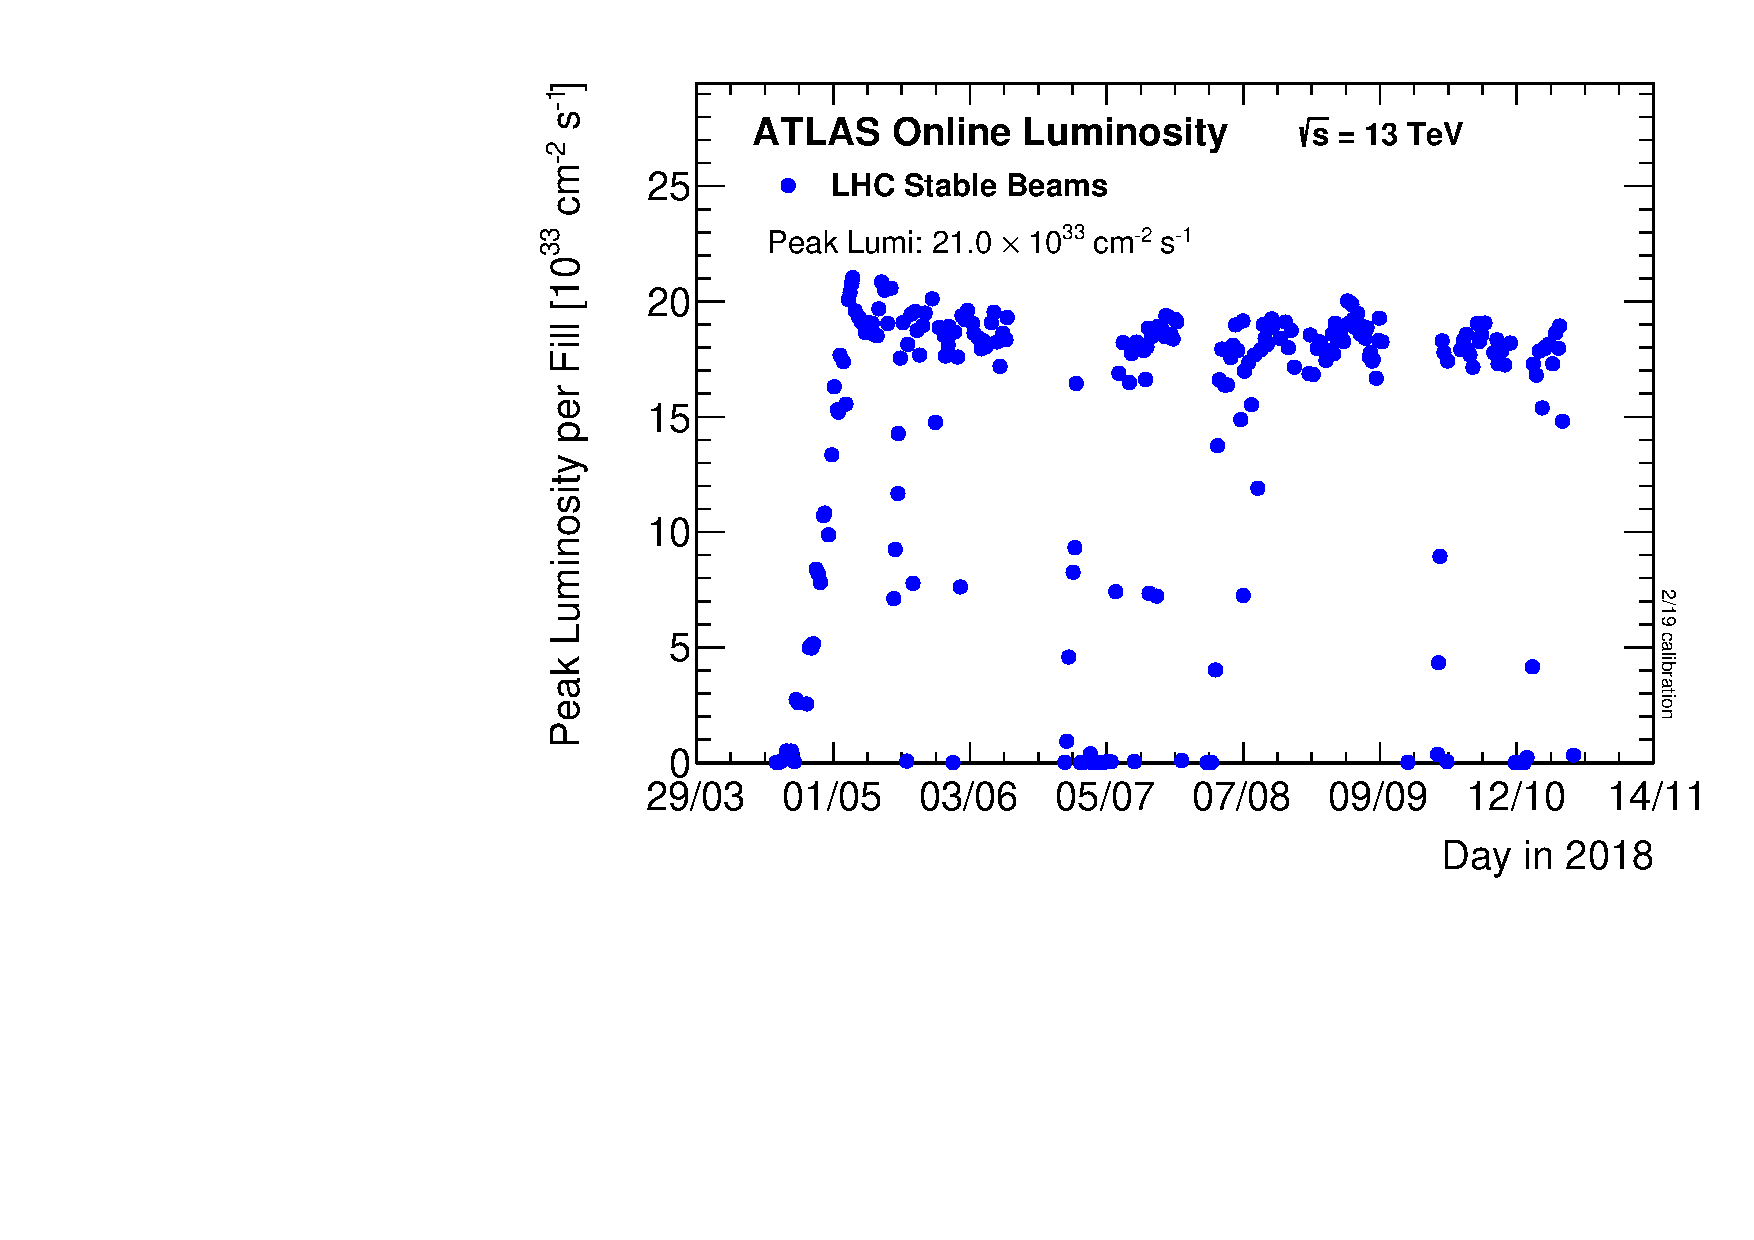
\includegraphics[width=0.5\textheight]{tesi_images/insta_lum_2018.pdf}
						\caption{The peak instantaneous luminosity delivered to ATLAS during stable beams for pp collisions at 13 TeV centre-of-mass energy per fill 2018}
						\label{fig:lum}
					\end{figure}
					
					For the nominal value of the luminosity $10^{34}$cm$^{-2}$s$^{-1}$ the total inelastic proton-proton cross-section is about 80 mb \cite{LHC introduction}  at $\sqrt{s} = 14$ TeV. Therefore, the event rate $R$, defined as the number of events produced per second by the pp interactions, is expected to be:
					$$
					R = \sigma L = 80 mb\times10^{34}cm^{-2}s^{-1} \simeq 10^{9}s^{-1}
					$$e 
					The number of events for each process is related to luminosity, it is proportional to the integrated luminosity shown in Figure \ref{fig:Integreted Luminosity}.
					
					\begin{figure}
						\centering
						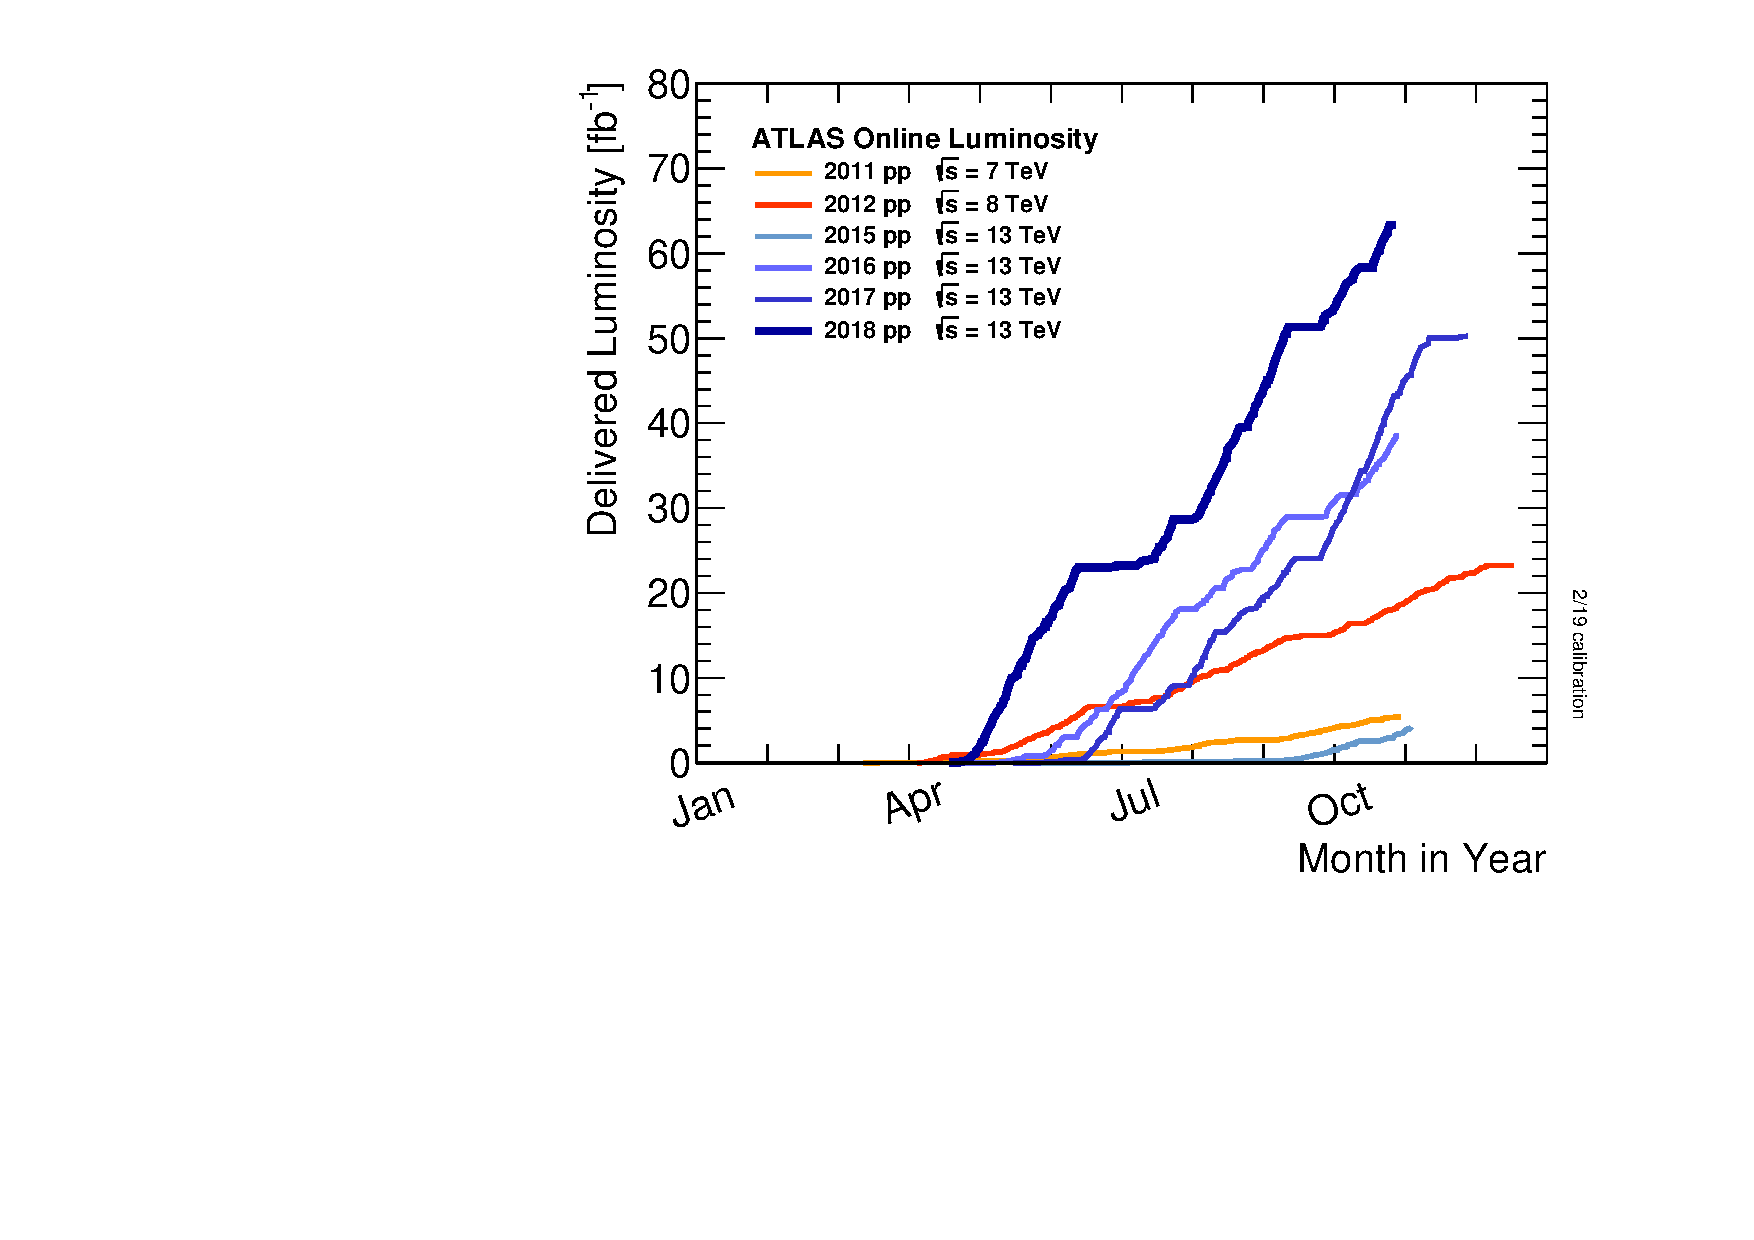
\includegraphics[width=0.5\textheight]{tesi_images/luminosity.pdf}
						\caption{Luminosity measured in inverse femtobarn versus time for 2011-2018 (p-p data only)}
						\label{fig:Integreted Luminosity}
					\end{figure}
					
					There are two types of pp collisions:
					\begin{itemize}
						\item \textbf{Soft collisions}: 
						they are the most of the collisions and they are large-distance collisions between the two incoming protons. They are called "soft" because the momentum transfer of the interaction is small. Due to this feature, particle scattering at large angle is suppressed and so, after collisions, particles have a large longitudinal momentum, but small transverse momentum ($<p_T>\simeq500$ MeV) relative to the beam line. The final states
						arising from such interactions are called minimum bias events.
						\item \textbf{Hard collisions}:
						monochromatic proton beams can be seen as beams of partons (quarks and gluons) with a wide band
						of energy. Occasionally, head-on collisions occur between two partons of the incoming protons. These are interactions at small distances, and therefore are characterised by large
						momentum transfers ("hard scattering"). In this case, particles in the final state can be produced at large angles with respect to the beam line (high $p_T$) and massive particles can be created.
						These are the interesting physics events at a collider but they are, however, rare compared to the soft interactions.
						
						In the hard-scattering interactions of quarks and gluons at a hadron collider, the effective centre-of-
						mass energy of the interaction ($\sqrt{\hat{s}}$) is smaller than the centre-of-mass energy of the machine ($\sqrt{s}$) and is given by: 
						$$ 
						\sqrt{\hat{s}} = \sqrt{x_ax_bs}
						$$
						where $x_a$ and $x_b$ are the fractions of the proton momentum carried by the two colliding partons. If $x_a \simeq x_b$, then the above relation becomes
						$$ 
						\sqrt{\hat{s}} \simeq x\sqrt{s}
						$$
						Therefore, in order to produce a particle of mass 100 GeV, two quarks (or gluons) which carry only 1\% of the proton momentum are needed ($x \sim 0.01$), whereas a particle of mass 5 TeV can only be produced if two partons with $x \sim 0.35$ interact. The momentum distributions of quarks and gluons inside the proton are called \textit{parton distribution functions}. % da fuonte p219
			\end{itemize}
		\section{ATLAS}	
			ATLAS \cite{ATLAS config} is one of two general-purpose detectors at the Large Hadron Collider. It investigates a wide range of physics, from the search for the Higgs boson to extra dimensions and particles that could make up dark matter. Although it has the same scientific goals as the CMS experiment, it uses different technical solutions and a different magnet-system design.
			\begin{figure}[H]
				\centering
				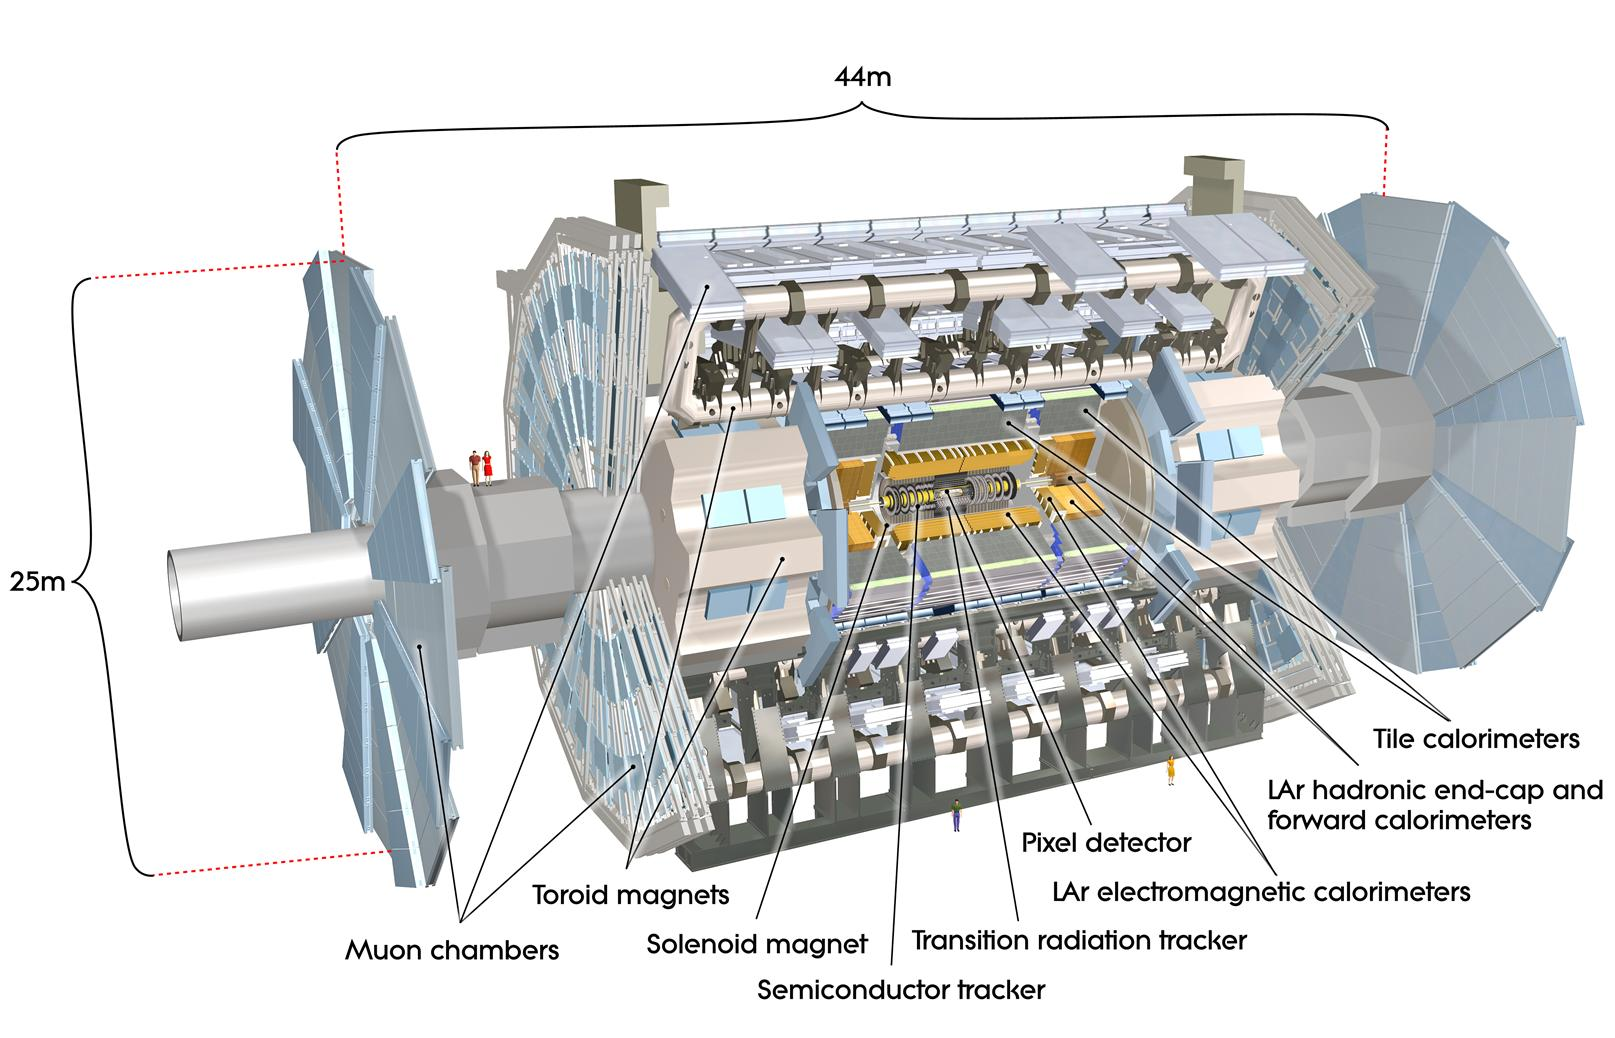
\includegraphics[width=0.6\textheight]{tesi_images/atlas_structure.jpg}
				\caption{ATLAS structure}
				\label{fig:ATLAS structure}
			\end{figure}
		
			Beams of particles from the LHC collide at the centre of the ATLAS detector making collision debris in the form of new particles, which fly out from the collision point in all directions. Six different detecting subsystems arranged in layers around the collision point record the paths, momentum, and energy of the particles, allowing them to be individually identified. A complex magnet system bends the paths of charged particles so that their momenta can be measured.
		
			The interactions in the ATLAS detectors create an enormous flow of data. To digest the data, ATLAS uses an advanced “trigger” system to tell the detector which events to record and which to ignore. Complex data-acquisition and computing systems are then used to analyse the recorded collision events. At 46 m long, 25 m high and 25 m wide, the 7000-tonne ATLAS detector is the largest volume particle detector ever constructed. 
				\subsection{Coordinate system}
					The origin of the coordinate system is set in the nominal point of interation. The beam direction defines the z-axis and the x-y plane is transverse to the beam direction. X-axis points from the interaction point to the centre of the LHC ring and Y-axis points upwards. The side-A of the detector is defined as that with positive z and side-C is that with negative z.
					
					Polar coordinate are also used: azimuthal angle $\phi$ is measured as usual around the beam axis, and the polar angle $\theta$ is the angle from the beam axis. Using $\theta$, pseudo rapidity is defined as $\eta= -\ln{\tan{\frac{\theta}{2}}}$. \\
					%(in the case of massive objects such as jets, the rapidity $y=\frac{1}{2}\ln{\frac{E+p_{z}}{E−p_{z}}}$ is used).%
					The transverse momentum $p_T$, the transverse momentum $E_T$, and the missing transverse energy $E_T^{miss}$ are defined in the x-y plane unless stated otherwise.  The distance $\Delta R$ in the pseudo rapidity-azimuthal angle space is defined as $\Delta R = \sqrt{\Delta \eta^2 + \Delta \phi^2 }$.
					\begin{figure}[H]
						\centering
						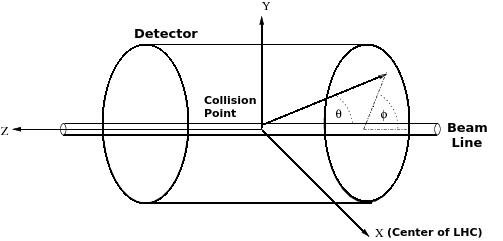
\includegraphics[width=0.3\textheight]{tesi_images/atlas_coord.jpeg}
						\caption{ATLAS coordinate system}
					\end{figure}
				\subsection{Magnet system}
					ATLAS features a unique hybrid system of four large superconducting magnets.  This magnetic system is 22 m in diameter and 26 m in length, with a stored energy of 1.6 GJ. \\
					\begin{figure}[H]
						\centering
						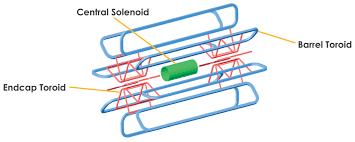
\includegraphics[width=0.5\textheight]{tesi_images/magnet_system_atlas.png}
						\caption{ATLAS magnet system}
					\end{figure}
					The  ATLAS  magnet  system consists of:
					\begin{itemize}
						\item a solenoid ("central solenoid"), which is aligned on the beam axis and provides a $2$ T axial magnetic field for the inner detector,  while minimising the radiative thickness in front of the barrel electromagnetic calorimeter;
						\item a  barrel  toroid and  two  end-cap  toroids, which  produce  a toroidal magnetic field of approximately $0.5$ T and $1$ T for the muon detectors in the central and end-cap regions, respectively.
					\end{itemize}
				\subsection{Inner detector}
					The ATLAS Inner Detector (ID) is the inner-most ATLAS layer and it is immersed in a 2 T solenoidal field. It is designed to provide hermetic and robust pattern recognition, excellent momentum resolution and both primary and secondary vertex measurements for charged tracks within the pseudorapidity range $|\eta|<2.5$. It also provides electron identification over $|\eta|<2.0$ up to energy of about 150 GeV. 
					\begin{figure}[H]
						\centering
						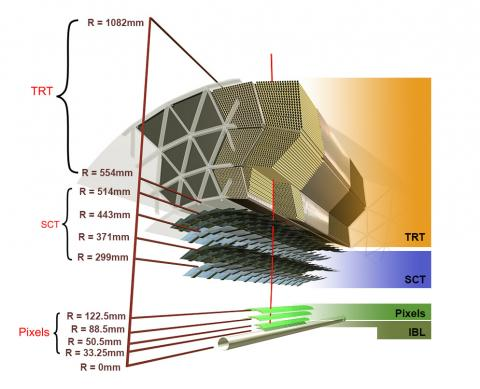
\includegraphics[width=0.45\textheight]{tesi_images/ID_structure.jpg}
						\caption{ATLAS Inner Detector structure}
					\end{figure}
					
					The ID is composed by three independent but complementary sub-detectors: 
					\begin{itemize}
						\item  \textbf{Pixel Detector}: \cite{ATLAS TDR} \cite{Inner Detector}
						it is  the  inner-most  part  of  the  ATLAS  tracking  system. It consists of 4 layers of barrel pixel detector and two end caps of three pixel disks each. The innermost pixel layer is a high-resolution pixel detector,  called Insertable B-Layer (IBL). The Pixel Detector sits inside the 2T solenoidal magnetic field and contributes to the charged particle tracking of the ATLAS Inner Detector in the pseudo rapidity range of $|\eta|<2.5$. Due to its high spatial resolution and 3-dimensional space-point measurement the Pixel Detector has a key-role in reconstruction of charged particle tracks.  The 4-Layer Pixel Detector is crucial in the reconstruction of primary and secondary vertices which is essential for example in the photon conversions reconstruction. 
						
						The single point resolution is 12 $\mu$m in the $R\cdot\phi$ and 75-112 $\mu$m in $z$ direction.
						\item \textbf{Semiconductor Tracker (SCT)}: \cite{ATLAS TDR} \cite{SCT}
						it consists of 61 $m^2$ of active silicon-strip detector modules and it is immersed in a 2 T solenoidal magnetic field. The  SCT  covers  the  radial  region  from  30  to  52  cm,  with  hermetic  azimuthal  coverage  out  to $|\eta|=2.5$. Four cylindrical layers in the central region form the “barrel” detector, and nine annular disks on each end of the barrel form the “endcaps”. The barrel layers are organized in 4 cylinders made of two layers of sensors glued back-to-back with a stereo angle of 40 $mrad$. The layout has been designed so that 4 space points can be provided for energetic charged particles will pass through at least four layers everywhere in the acceptance region. 
						
						The single point resolution is 16 $\mu$m in the $R\cdot\phi$ and 580 $\mu$m in $z$ direction.
						\item \textbf{Transition Radiation Tracker (TRT)}: \cite{ATLAS TDR} \cite{TRT}
						it is the outmost of the three tracking subsystems of the ATLAS Inner Detector. The TRT is a straw-tube tracker. When a charged particle traverses the TRT, it ionises the gas inside the straws. The resulting free electrons drift towards the wire, where they are amplified and read out.\\
						The spaces between the straws are filled with polymer fibres (barrel) and foils (endcaps) to create transition radiation, which may be emitted by highly relativistic charged particles as they traverse a material boundary.   This effect depends on the relativistic factor $\gamma=E/m$ and is strongest for electrons, so it could be a discriminating factor.
						This design  makes the TRT complementary to  the silicon-based tracking devices:  the intrinsic single-point resolution of 130 $\mu$m is larger than that of the silicon trackers, but this is compensated by the large number of hits per track (typically more than 30). 
					\end{itemize}
					The overall momentum resolution is:
					$$
					\frac{\sigma_{p_T}}{p_T} = 0.05\% p_T \oplus 1\%
					$$
				\subsection{Calorimetry system}
					\cite{Calo intro}Calorimeters measure the energy a particle loses as it passes through the detector, so the energy of all charged and neutral particles. It is usually designed to stop  or “absorb” the particles coming from a collision, forcing them to deposit all of their energy within the detector. Calorimeters typically consist of layers of “passive” or “absorbing” high-density material interleaved with layers of an “active” medium such as solid lead-glass or liquid argon. Calorimeters are designed to stop most known particles except muons and neutrinos.
					\begin{figure} [H]
						\centering
						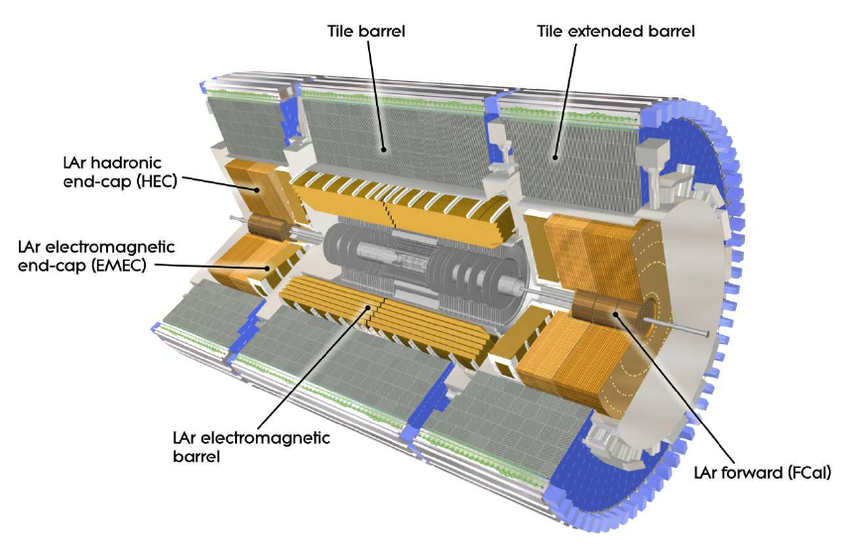
\includegraphics[width=.6\textwidth]{tesi_images/calorimeters.png} 
						\caption{ATLAS calorimetry system}
						\label{fig:Calorimetry}
					\end{figure}
					The components of the ATLAS calorimetry system are: \cite{ATLAS TDR} \cite{Calorimetry}
					\begin{itemize}
						\item \textbf{electromagnetic calorimetry}:
						the ATLAS EM calorimeter is a lead–liquid argon (LAr) sampling detector with accordion-shaped electrodes and lead absorber plates over its full coverage. The calorimeter is divided into a Barrel part and two End-Caps. Each End-Cap is divided into two coaxial wheels: an outer wheel and an inner wheel covering, respectively, $1.375<|\eta|<2.5$ and $2.5<|\eta|<3.2$. The absorber lead thickness is constant over large areas. The argon gap thickness is constant in the Barrel but changing with the radius in the End-Cap.
						In the range $|\eta|<1.8$, the calorimeter is preceded by a presampler to recover the energy lost in the upstream material (cryostat, super-conducting coil, inner detector, etc.). The typical energy resolution is:
						$$ 
						\frac{\sigma(E)}{E} = \frac{10\%}{\sqrt{E}} \oplus 0.7\%
						$$
						
						\begin{figure}[h!]
							\centering
							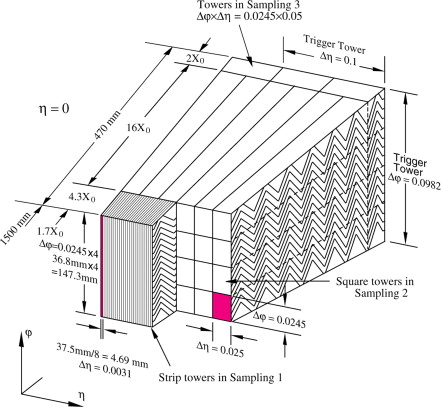
\includegraphics[width=.6\textwidth]{tesi_images/calo_struct.jpg}
							\caption{The EM calorimeter accordion geometry}
							\label{fig:calo struct}
						\end{figure}
						\begin{table}[h!]
							\centering
							\begin{tabular}{cc}
								\toprule[1.5pt]
								\textbf{Layer} & \textbf{Granularity ($\Delta\eta \times \Delta\phi$)} \\
								\midrule
								Presampler & $0.025 \times 0.1$ \\
								Layer 1 & $0.0031 \times 0.1$ \\
								Layer 2 & $0.025 \times 0.0245$ \\
								Layer 3 & $0.05 \times 0.245$ \\
								\bottomrule[1.5pt]
							\end{tabular}
								\caption{Granularity of different layers of the EM calorimeter}\label{tab:granularity}
							
						\end{table}
										
						\item \textbf{hadronic calorimeters}:
						in the range $|\eta|<1.6$, the ATLAS hadronic calorimeter is an iron-scintillating tiles calorimeter. The Hadronic Tile calorimeter is located behind the solenoid coil and the EM calorimeter. It is a sampling calorimeter using iron as absorber material and scintillating tiles as active material. The Hadronic End-Cap calorimeter (HEC) is an LAr sampling calorimeter using copper and tungsten as passive material. It provides full coverage for $1.5<|\eta|<3.2$. The typical resolution for jets is:
						$$ 
						\frac{\sigma(E)}{E} = \frac{50\%}{\sqrt{E}} \oplus 3\%
						$$
						\item \textbf{forward calorimeters} (FCal):
						in the forward region ($3.1<|\eta|<4.9$), calorimetry is done by another type of LAr calorimeter. The Forward Calorimeter (FCAL) consists of copper (Em) or tungsten (Had) rods parallel to the beam axis inside an outer tube with 250 $\mu$m liquid argon gap in between. The typical resolution for jets is:
						$$ 
						\frac{\sigma(E)}{E} = \frac{100\%}{\sqrt{E}} \oplus 10\%
						$$
					\end{itemize}
		
		
				\subsection{Muon spectrometer}
					\cite{Muon system}The  muon  spectrometer  forms  the  outer  part  of  the  ATLAS  detector  and occupies by far the largest volume. It was designed to serve two purposes: an independent muon trigger and high quality stand-alone muon reconstruction over a wide range in transverse momentum, pseudo-rapidity ($|\eta|<2.4$ trigger, $|\eta|<2.7$ momentum) and azimuthal angle. This is achieved by the use of a large toroidal magnet system together with trigger and high precision tracking chambers.
					
					The magnet system of the muon spectrometer consists of three air-core toroids. Each toroid is build up of eight super conducting coils assembled in a radial configuration. Accurate knowledge of the field is required in order not to degrade the momentum resolution. During ATLAS running a large number of magnetic field sensors will measure the local field ensuring a knowledge of the bending power with a precision better than 0.3\%. 
					
					Figure \ref{fig:ATLAS muon detector}a shows the transverse view of the barrel part of the muon spectrometer. In the barrel a particle typically traverses three measurement planes. The inner most stations are situated directly after the hadronic calorimeter, just before the toroidal magnetic region. They are equipped with MDT chambers which allow a high precision measurement of the muon trajectory. The second layer of stations is situated in the magnet. The stations in this layer consist of a combination of one MDT chamber and two Resistive Plate Chambers (RPC). A third layer of stations is located just outside the magnetic field. The outer stations are formed by a combination of a MDT chamber and a RPC.
					
					The design of the muon system in the end-caps is different as it is not possible to install stations inside the end-cap magnets and the background rate is much higher. In the end-cap, the first layer of stations sits in front of the magnet. The region closest to the beam pipe, where the background counting rates are highest, is equipped with Cathode Strip Chambers (CSC) instead of MDT chambers because of their higher rate capability. MDT chambers provide the remaining coverage. Thin Gap Chambers(TGC) are installed providing the trigger signal. The second station layer is installed behind the end-cap magnet and is equipped with one layer of MDT chambers and two layers of TGCs. The outer station layer is equipped with MDT chambers.
					
					The typical energy resolution is resolution is 2-3\% to 10 GeV and goes up to 10\% to 1 TeV.
					\begin{figure} [H]
						\centering
						\subfloat[][\emph{Transverse xy-view of the ATLAS muon detector}]{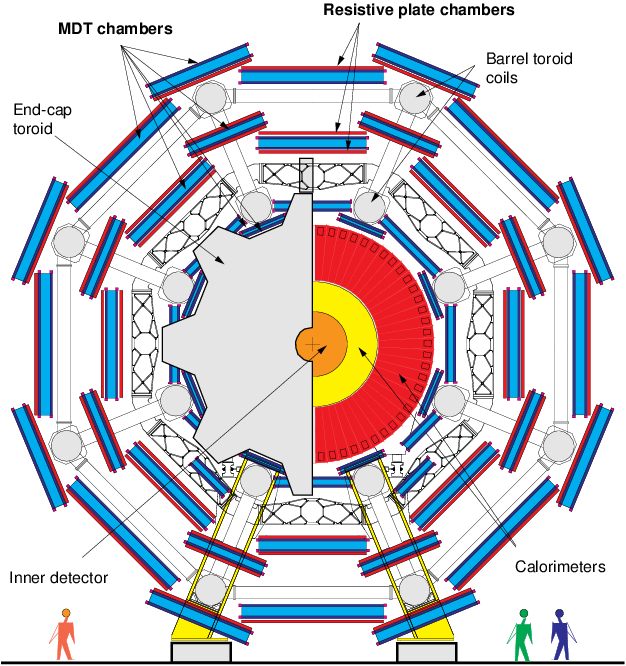
\includegraphics[width=.3\textwidth]{tesi_images/muon_spectrometer.png}} \quad
						\subfloat[][\emph{3D view of the ATLAS detector}]{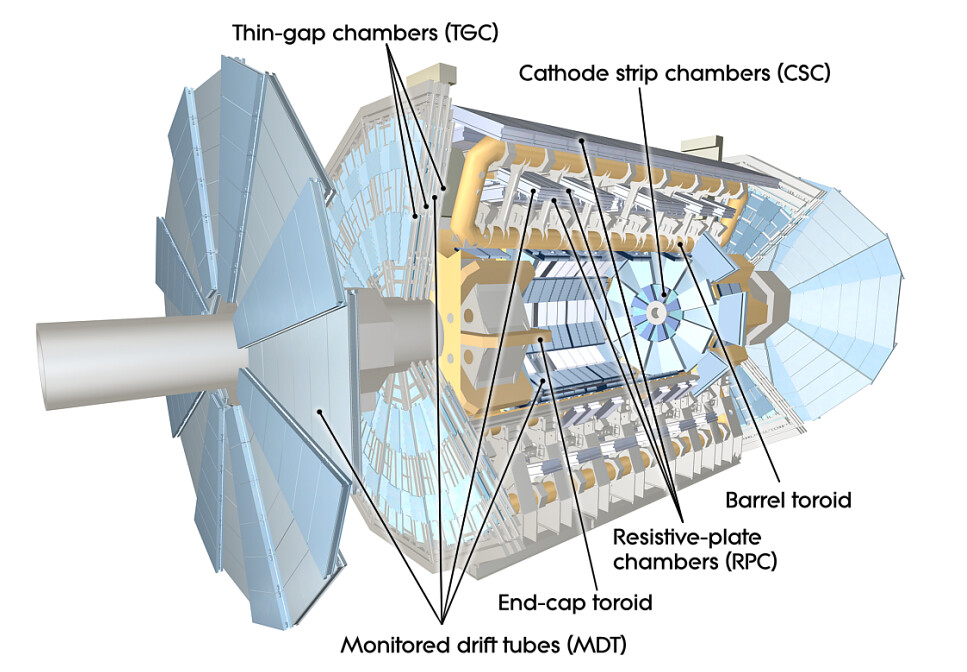
\includegraphics[width=.45\textwidth]{tesi_images/3D-muon.jpg}} 
						\caption{ATLAS muon detector}
						\label{fig:ATLAS muon detector}
					\end{figure}
				
				\subsection{Trigger system}
					\cite{Trigger intro}ATLAS is designed to observe up to 1.7 billion proton-proton collisions per second, with a combined data volume of more than 60 million megabytes per second. However, only some of these events will contain interesting characteristics that might lead to new discoveries. To reduce the flow of data to manageable levels, ATLAS uses a specialised two-level online event selection system - the Trigger System - which selects events with distinguishing characteristics that make them interesting for physics analyses. The Trigger System selects approximately 1000 of the 1.7 billion collisions that occur each second in the centre of the ATLAS detector. 
				
					The two independent levels (Figure \ref{fig:Trigger system}) are, a hardware-based first level (L1) and a software-based high level trigger (HLT) \cite{Trigger system}. 
					\begin{itemize}
						\item The L1 trigger is implemented in fast custom-made electronics and runs with a fixed latency of 2.5$\mu$s. L1 reduces the event rate from the LHC interaction rate of 40 MHz to $\approx$ 100 kHz. Up to 512 decision items are built, based on Regions of Interest (RoI) in $\eta/\varphi$ retrieved from the muon (L1Muon) and calorimeter (L1Calo) systems. The L1 trigger decision is formed by the Central Trigger Processor (CTP). The L1Topo trigger, which is a system introduced for Run-2, performs selections based on geometric or kinematic association between trigger objects received from L1Calo or L1Muon. 
						
						\item In the HLT, offline-like reconstruction algorithms run in a large farm of $\approx$ 40.000 processor cores and a decision is formed typically within 300 ms. The HLT is a software trigger providing typically 2500 independent trigger chains. These are sequences of offline-like algorithms executed within the L1 RoIs. Furthermore, full-event reconstruction is possible at the HLT. Events accepted by the HLT are written into different data streams to be used for physics analysis, trigger level analysis, monitoring or detector calibration. Depending on the datastream, the full event or only partial event information is written out, allowing for higher rates without consuming a significant amount of the available bandwidth.
					\end{itemize}
					
					\begin{figure}[h!]
						\centering
						\subfloat[]{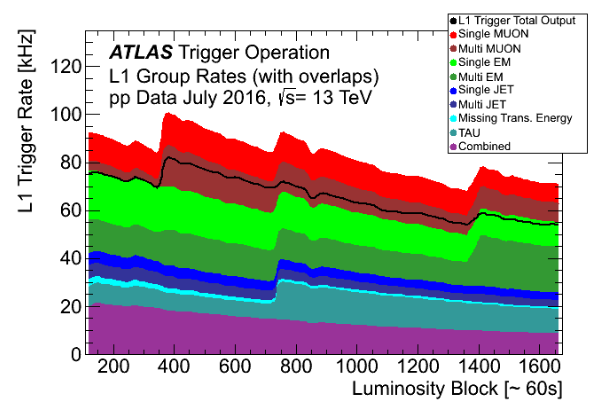
\includegraphics[width=.6\textwidth]{tesi_images/L1.png}} \quad
						\subfloat[]{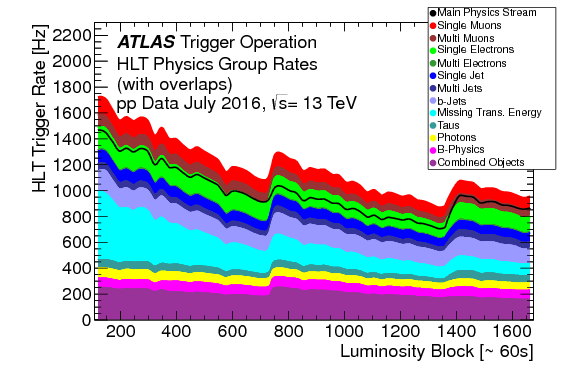
\includegraphics[width=.6\textwidth]{tesi_images/HLT.png}} 
						\caption{L1 (a) and HLT (b) physics trigger rates grouped by trigger signatures as a function of theluminosity block number, in a fill taken in July 2016 with a peak instantaneous luminosity of $1.2 \times 10^{34}$cm$^{-2}$s$^{-1}$}
						\label{fig:Trigger system}
					\end{figure}
		\section{ATLAS Physics Programme}
			\cite{STD Model}ATLAS explores a range of physics topics, with the primary focus of improving our understanding of the fundamental constituents of matter and their interactions. Currently this is well described by the so called Standard Model (SM), a quantum field theory based on SU2$\otimes$U1$\otimes$SU3.
			ATLAS is studying the processes predicted by the SM such as \textit{w,z} and \textit{top} production and compare the measured cross section with the model predictions.
			\begin{figure}[h!]
				\centering
				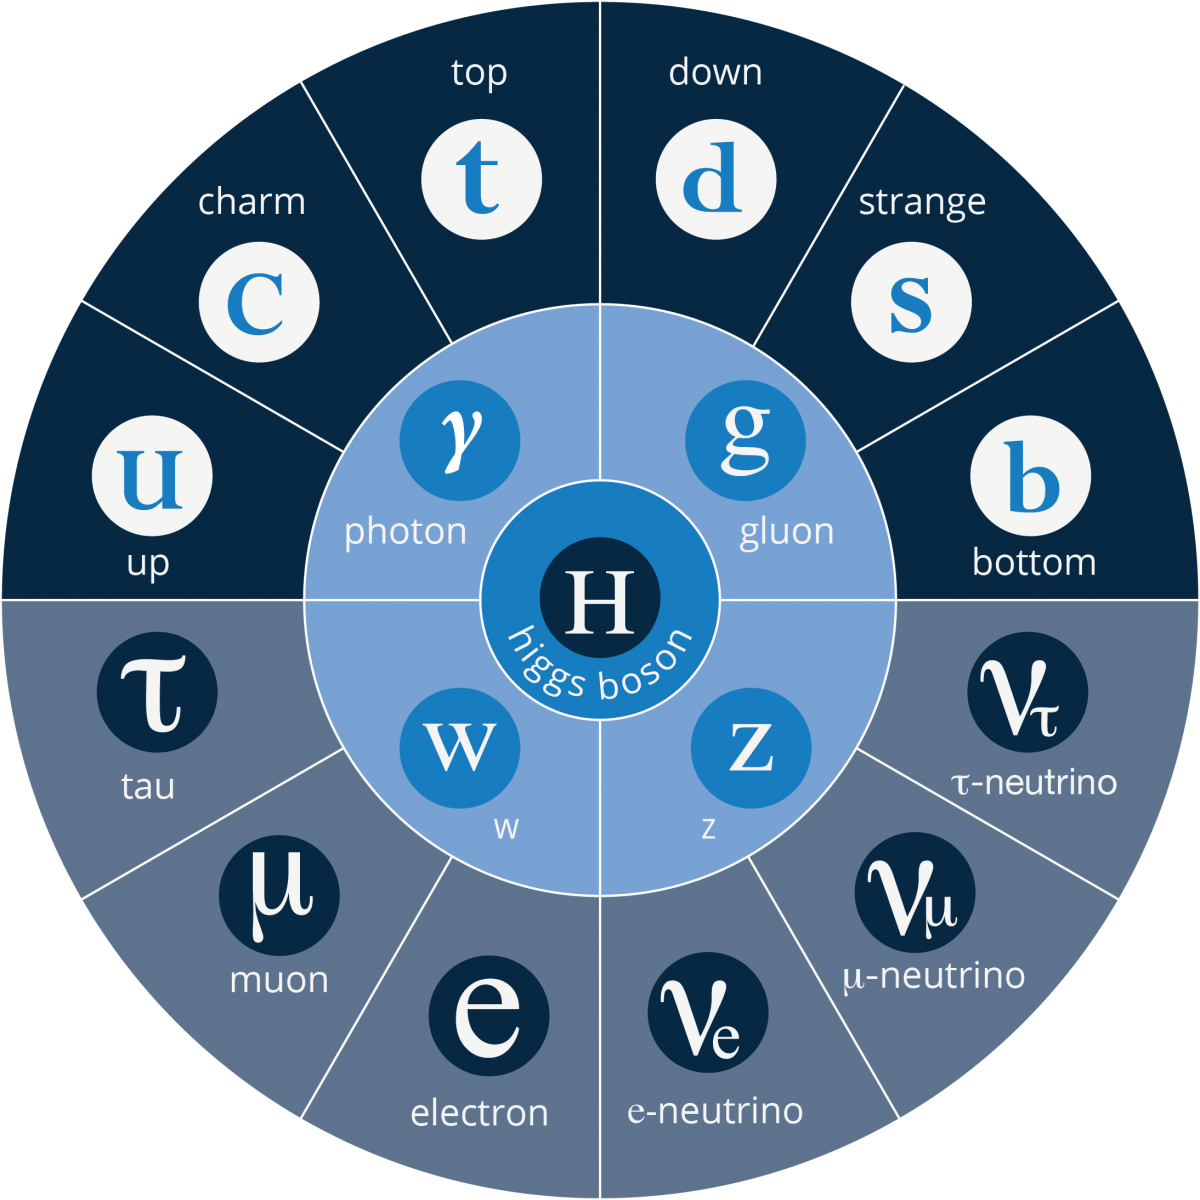
\includegraphics[width=.3\textwidth]{tesi_images/STD_model.png}
				\caption{Particles in the Standard Model}
				\label{fig:STD model}
			\end{figure}
			ATLAS is also useful in the study of forces that govern their interactions. Indeed, the Standard Model also describes the fundamental forces of Nature and how they act between fundamental particles. In addition ATLAS is looking for new physics signatures like the ones proposed in Supersymmetry models, where forces combine with very high energies.
			
			Due to the Proton-proton and heavy-ion collisions, LHC  recreate the conditions immediately following the Big Bang when the Universe was governed by high-energy particle physics and later by a primordial soup of quarks and gluons, and allow ATLAS to study fundamental questions such as the Brout-Englert-Higgs field or Dark Matter.
			
			One of the most important ATLAS discoveries is the proof of the existence of the Higgs boson. On 4 July 2012, the ATLAS and CMS \cite{CMS} experiments at CERN announced that they had independently observed a new particle in the mass region of around 126 GeV: a boson consistent with the Higgs boson \cite{Higgs}.
				
	\chapter{Electron and photon reconstruction}
		Events with electrons and photons in the final state are important signatures for many physics analyses envisaged at the LHC. Their reconstruction mainly  exploits data coming from the electromagnetic calorimeter (clusters) and the Inner Detector (ID) systems (tracks) \cite{El ph intro}\cite{El ph reco}: 
		\begin{itemize}
			\item an electron is defined as an object consisting of a cluster built from energy deposits in the
			calorimeter (supercluster) and a matched track (or tracks);
			\item a  converted photon is a cluster matched to a conversion vertex (or vertices), and an unconverted photon is a cluster matched to neither an
			electron track nor a conversion vertex. About 20\% of photons at low $|\eta|$ convert in the ID, and up to about 65\% convert at $|\eta| \simeq 2.3$.
		\end{itemize}
		The reconstruction  with $|\eta| < 2.5$ is based on an algorithm. It first prepares the tracks and clusters it will use. It selects clusters of energy deposits measured in topologically connected EM and hadronic calorimeter cells, denoted topo-clusters. These clusters are matched to ID tracks, which are re-fitted accounting for bremsstrahlung. The algorithm also builds conversion vertices and matches them to the selected topo-clusters. The electron and photon supercluster-building steps then run separately using the matched clusters as input. After applying initial position corrections and energy
		calibrations to the resulting superclusters, the supercluster-building algorithm matches tracks to the electron superclusters and conversion vertices to the photon superclusters. The electron and photon
		objects to be used for analyses are then built, their energies are calibrated, and discriminating
		variables used to separate electrons or photons from background are added.
		
		\section{The topo-cluster reconstruction}
			The topo-cluster reconstruction algorithm begins by forming proto-clusters in the EM and hadronic calorimeters using a set of noise thresholds in which the cell initiating the cluster is EM required to have significance $|\zeta_{cell}^{EM}| \geq 4$ where 
			$$
			\zeta_{cell}^{EM} = \frac{E_{cell}^{EM}}{\sigma_{cell}^{EM}}
			$$		
			$E_{cell}^{EM}$ is the energy cell at the EM scale and $\sigma_{cell}^{EM}$ is the expected cell noise, which includes the known electronic noise and an estimate of the pile-up noise corresponding
			to the average instantaneous luminosity expected for Run 2. In order to suppres the formation of noise cluster, in this initial stage, cells from the presampler and the first LAr EM calorimeter layer are excluded from initiating proto-clusters.
			An important role is played by the neighbouring cells. If they have a significance $|\zeta_{cell}^{EM}| \geq 2$, these cells are collected by proto-cluster. Each neighbour cell passing the threshold of $|\zeta_{cell}^{EM}| \geq 2$ becomes a seed cell in the next iteration, collecting each of its neighbours in the proto-cluster. If two proto-clusters EM contain the same cell with $|\zeta_{cell}^{EM}| \geq 2$ above the noise threshold, these proto-clusters are merged. A crown of nearest-neighbour cells is added to the cluster independently on their energy ($|\zeta_{cell}^{EM}| \geq 0$). This set of thresholds is commonly known as ‘4-2-0’ topo-cluster reconstruction.\\
			Energy becomes an important feature when a cell has $|E_{cell}^{EM}| > 500$ MeV. A cell with this energy, at least four neighbours, and when none of the neighbours has a larger signal, is a local maximum. Proto-clusters with two or more local maxima are split into separate clusters.
			
			%Electron and photon reconstruction starts from the topo-clusters but only uses the energy from cells in the EM calorimeter, except in the transition region of $1.37<|\eta|<1.63$, where the energy measured in the presampler and the scintillator between the calorimeter cryostats is also added.%
		
		\section{Track reconstruction}
		Track finding is one of the most challenging tasks in reconstructing events from proton-proton  collisions  recorded  by  the  ATLAS  detector. The process consists in finding a track in the ID which can be matched to the energy clusters. The ID track reconstruction consists of several sequences with different strategies and the main sequence is referred to as inside-out track finding: \cite{ID reco alg}
		\begin{itemize}
			\item \textbf{Space point formation}: the initial step of the ID reconstruction consists of the cluster and drift circle creation and the transformation of clusters in the silicon detectors into 3D space points. Clusters are formed by finding connected cells in
			the pixel and strip detectors. \cite{Track reco}From these clusters, three-dimensional measurements referred to as space-points are created. In the pixel detector, each cluster equates to one space-point, while in the SCT, clusters from both stereo views of a strip layer must be combined to obtain a three-dimensional measurement. 
			
			\item \textbf{Space point seeded track finding}: track seeds are formed from sets of three space-points in the silicon-detector layers. \cite{ID reco alg} Seeds can be built from space points in the pixel detector only (referred to as PPP seeds), the strip detector only (SSS) or any mixed setup (PSS,PPS). To reduce the number of potential seeds, initial cuts are applied and dedicated care is taken not to
			extensively use space points in multiple seeds. Seeds that pass the initial requirements are then input to a track finding algorithm that uses a combinatorial Kalman filter technique and aims to complete the track candidates within the silicon detector.
			
			\item \textbf{Ambiguity solving}: track candidates are then further processed in an ambiguity solving
			module that aims to eliminate track candidates from random hit combinations (often
			referred to as "fakes") or track duplicates, which can be identified by measurements that are shared with other track candidates. The ambiguity solving relies on a scoring function applying positive scores for unique measurements and good fit quality, while penalising missing measurements where they would be expected (also called holes) or shared measurements with other track candidates.
			
			\item \textbf{TRT extension}: tracks that successfully pass the ambiguity solving stage and are within the coverage of the TRT detector are then extended into the TRT and completed for measurements in the outermost tracking detector. A successful TRT extension increases the
			momentum resolution significantly by exploiting the longer lever arm for field integration.
		\end{itemize}
		
		\section{Track-cluster matching and photon conversion reconstruction}
			\cite{El ph reco} After cluster and track reconstruction, the next step is the track-cluster matching. Fixed-size clusters in the calorimeter are used to create regions-of-interest (ROIs) and tracks intersecting
			these regions are considered loosely matched to the cluster. Track candidates are then fitted with the global $\chi^2$ fitter. The loosely matched, re-fitted tracks are then matched to the EM topo-clusters (with requirements, see \cite{El ph reco}).
			If multiple tracks are matched to a cluster, they are ranked in order to choose the best one. To assign the rank, tracks are compared on the number of hits in the Pixel and SCT detectors. Another rank characteristic is $\Delta R$: tracks with a better $\Delta R$ match between the track and cluster coordinates are preferred. So the highest-ranked track is used to define the reconstructed electron properties.
			
			Tracks loosely matched to fixed-size clusters serve as input to the reconstruction of the conversion vertex. Both tracks with silicon hits and tracks reconstructed only in the TRT are used for the conversion reconstruction. Two-track conversion vertices are reconstructed from two opposite-charge tracks forming a vertex consistent with that of a massless particle, while single-track vertices are essentially tracks without hits in the innermost sensitive layers. To increase the converted-photon purity, the tracks used to build conversion vertices must have a high probability to be electron tracks as determined by the TRT. The requirement is loose for Si tracks but tight for TRT tracks used to build double-track conversions, and even tighter for tracks used to build single-track conversions. 
			
			The conversion vertices are then matched to the EM topo-clusters. Using tracks with silicon hits, a conversion vertex is considered matched if extrapolated tracks
			match the cluster to within $|\Delta \eta|$ and $|\Delta \phi|$ < 0.05. With TRT only tracks these requirements are looser.
			If there are multiple conversion vertices matched to a cluster, double-track conversions with two silicon tracks are preferred over other double-track conversions, followed by single-track conversions. Within each category, the vertex with the smallest
			conversion radius is preferred.
			
			
		\section{Supercluster reconstruction}
		The reconstruction of electron and photon superclusters proceeds independently, each in two stages \cite{El ph reco}:
		\begin{enumerate}
		\item in the first stage, EM topo-clusters are tested for use as seed cluster candidates, which form the basis of superclusters; 
		\item in the second stage, EM topo-clusters near the seed candidates are identified as satellite cluster candidates, which may emerge from bremsstrahlung radiation or topo-cluster splitting.
		\end{enumerate}
		Superclusters are built through various steps:
		\begin{itemize}
		\item the initial list of EM topo-clusters is
		sorted according to descending $E_T$ , calculated using the EM energy.
		\item the clusters are tested one by one in the sort order for use as seed clusters. There are two seed's kind:
			\begin{enumerate}[label=\roman*.]
				\item electron supercluster seed: a cluster with a minimum $E_T$ of 1 GeV and matched to a track with at least four hits in the silicon tracking detectors.
				\item photon supercluster seed: a cluster with $E_T$ greater
				than 1.5 GeV with no requirement made on any track or conversion
				vertex matching.
			\end{enumerate}
		A cluster cannot be used as a seed cluster if it has already been added as a satellite cluster to another seed cluster.
		\item if a cluster meets the characteristics of the previous point, the algorithm attempts to find satellite clusters, using the process summarized in figure \ref{fig:super_cl}.
		\begin{figure}
			\centering
			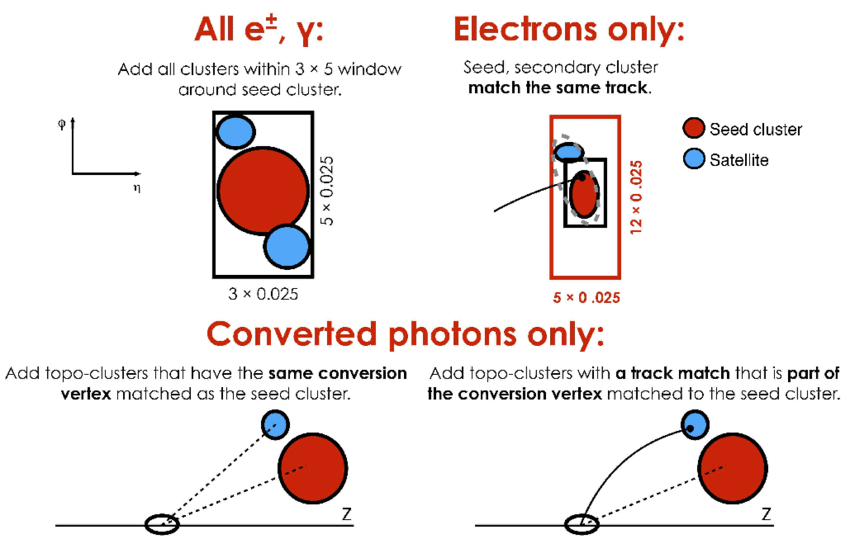
\includegraphics[width=0.45\textheight]{tesi_images/super_cluster.png}
			\caption{Diagram of the superclustering algorithm for electrons and photons. Seed clusters are shown in
			red, satellite clusters in blue.}
			\label{fig:super_cl}
		\end{figure}
		For both electrons and photons, a cluster is considered a satellite if it falls within a window of $\Delta\eta \times \Delta\varphi = 0.075 \times 0.125$ around the seed cluster barycentre, as these cases tend to represent secondary EM showers originating from the same initial electron or photon.
		For electrons, this window could be larger, $\Delta\eta \times \Delta\varphi = 0.125 \times 0.300$, and its ‘best-matched’ track is also the best-matched track for the seed cluster. For photons with conversion vertices made up only of tracks containing silicon hits, a cluster is added as a satellite if its best-matched (electron) track belongs to the conversion vertex matched to the seed cluster. These steps rely on tracking information to discriminate distant radiative photons or conversion electrons from pile-up noise or other unrelated clusters. \\
		The seed clusters with their associated satellite clusters are called superclusters.
		
		\item The final step in the supercluster-building algorithm is to assign calorimeter cells to a given supercluster. Only cells from the presampler and the first three LAr calorimeter layers are considered, except in the transition region of $1.4 < |\eta| < 1.6$, where the energy measured in the scintillator between the calorimeter cryostats is also added. To limit the superclusters’ sensitivity to pile-up noise, the size of each constituent topo-cluster is restricted to a maximal width of 0.075 or 0.125 in the $\eta$ direction in the barrel or endcap region, respectively. Because the magnetic field in the ID is parallel to the beam-line, interactions between the electron or photon and detector material generally cause the EM shower to spread in the $\varphi$ direction, so the restriction in $\eta$ still generally allows the electron or photon energy to be captured. No restriction is applied in the $\varphi$-direction.	
		\end{itemize}
		\section{Creation of electrons and photons for analysis}
		\cite{El ph reco}After the electron and photon superclusters are built, tracks are matched to electron superclusters and conversion vertices to photon superclusters. Then the analysis-level
		electrons and photons are created. Because electron and photon superclusters are built independently, a given seed cluster can produce both an electron and a photon. In such cases, the procedure
		presented in figure \ref{fig:el_ph_analisi} is applied. The purpose is that if a particular object can be easily identified only as a photon (a cluster with no good track attached) or only as an electron (a cluster with a good track attached and no good photon conversion vertex), then only a photon or an electron object is created for analysis; otherwise, both an electron and a photon object are created. Furthermore, these cases are marked explicitly as ambiguous, allowing the final classification of these objects to be determined based upon the specific requirements of each analysis.
		\begin{figure}
			\centering
			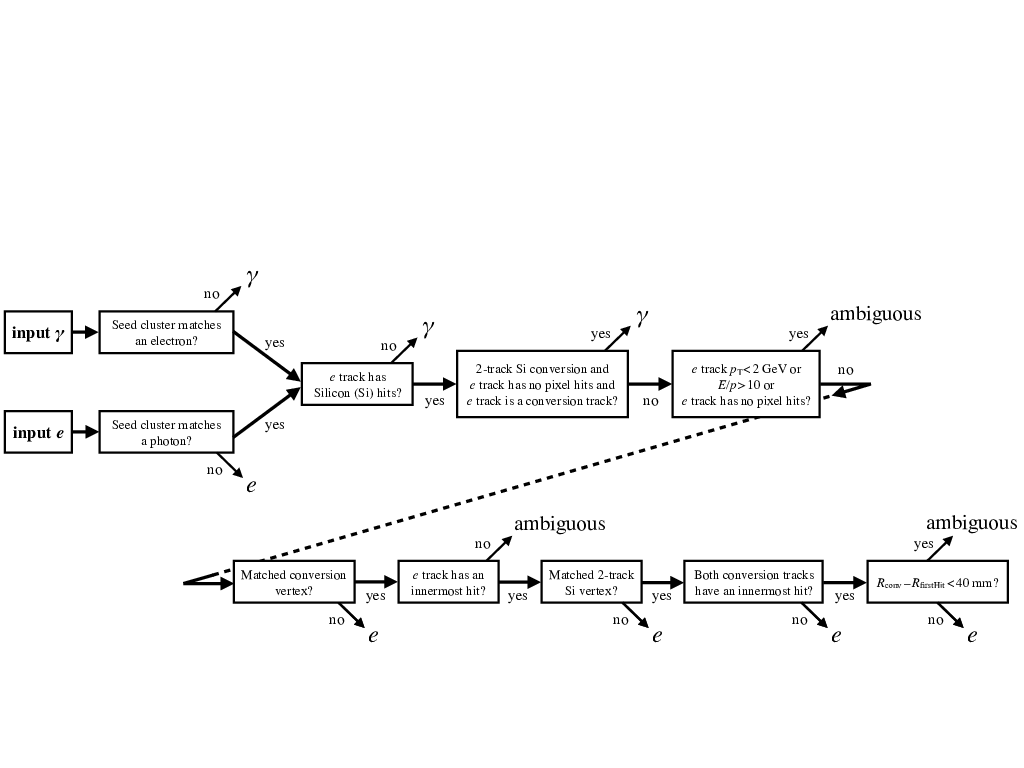
\includegraphics[width=0.45\textheight]{tesi_images/el_ph_analisi.png}
			\caption{Flowchart showing the logic of the ambiguity resolution for particles initially reconstructed both as electrons and photons.}
			\label{fig:el_ph_analisi}
		\end{figure}
	
		\section{Identification}
		\cite{Identification}Excellent electron and photon identification capabilities are crucial for many aspects of the ATLAS physics program, from standard model measurements (including Higgs boson) to new physics searches. The identification of prompt photons and the rejection of backgrounds, mostly coming from photons from hadron decays, relies on the high granularity of the ATLAS calorimeter. Electron identification is based on a likelihood (LH) discrimination to separate isolated electron candidates from candidates originating from photon conversions, hadron misidentification and heavy flavor decays. 
			\subsection{Elettron identification}
			\cite{El ph reco}The quantities used in the electron identification are chosen according to their ability to discriminate prompt isolated electrons from energy deposits from hadronic jets, from converted photons and from genuine electrons produced in the decays of heavy-flavour hadrons. The variables can be
			grouped into properties of (Table \ref{tab:el parameters}):
			\begin{itemize}
				\item the primary electron track, which is required to fulfil a set of quality requirements, namely hits in the two inner tracking layers closest to the beam line, as well as a number of hits in the silicon-strip detectors. The transverse impact parameter of the track and its significance are used to construct
				the likelihood discriminant.
				\item the lateral development of the electromagnetic shower, which is characterized with variables calculated separately in the first and second layer of the electromagnetic calorimeter. To reject clusters from multiple incident particles, $w_{s tot}$ is used. The lateral shower development is measured with $R_{\varphi}$ and $R_{\eta}$.
				\item the longitudinal development of the electromagnetic shower, for them the numbers of cells contributing to the energy
				measurement in each layer are chosen dynamically in the supercluster approach, compared with fixed numbers of cells in fixed-size clusters. The supercluster approach inherently suppresses noise in the calorimeter cells, resulting in lower values and narrower distributions. The electron
				identification uses $f_1$ and $f_3$.
				\item the spatial compatibility of the primary electron track with the reconstructed cluster, which are matched using $\Delta\eta_1$ and $\Delta\phi_{res}$. 
			\end{itemize}
			\begin{table}
				
				\begin{tabular}{lp{8cm}c}
					\toprule[1.5pt]
					\textbf{Type} & \textbf{Description} & \textbf{Simbol}\\
					\midrule
					\multirow[t]{5}{*}{Hadronic leakage} 
					& {- Ratio of $E_T$ in the first layer of the hadronic calorimeter to $E_T$ of the EM calorimeter (in the pseudorapidity range $|\eta| < 0.8$ or $|\eta| > 1.37$)} & $R_{had1}$   \\ 
					& - Ratio of $E_T$ in the first layer of the hadronic calorimeter to $E_T$ of the EM calorimeter (in the pseudorapidity range $0.8 < |\eta| < 1.37$) & $R_{had}$  \\
					\midrule
					Layer 3 of the EM calorimeter & Ratio of the energy in the back layer to the total energy in the EM calorimeter. This variable is only used below 100 GeV because it is known to be inefficient at high energies. & $f_3$ \\
					\midrule
					\multirow[t]{5}{*}{Layer 2 of the EM calorimeter}
					& - Lateral shower width $\sqrt{(\sum_{i}E_i\eta_i^2)/(\sum_{i}E_i) - ((\sum_{i}E_i\eta_i)/(\sum_{i}E_i))^2}$ ,where
					$E_i$ is the EM calorimeter energy and $\eta_i$ is the pseudorapidity of cell i and the sum is calculated within a window of 3 × 5 cells & $w_n^2$ \\
					& - Ratio of the energy in 3 × 3 cells over the energy in 3 × 7 cells
					centered at the electron cluster position & $R_\phi$ \\
					& - Ratio of the energy in 3 × 7 cells over the energy in 7 × 7 cells centered at the electron cluster position & $R_\eta$ \\
					\midrule
					\multirow[t]{3}{*}{Layer 1 of the EM calorimeter}
					& - Shower width, $\sqrt{(\sum_{i}E_i(i-i_{max})^2)/(\sum_{i}E_i)}$ where i runs over all strips in a window of $\Delta\eta \times \Delta\varphi \sim 0.0625 \times 0.2$ , corresponding typically to 20 strips in $\eta$, and $i_{max}$ is the index of the highest-energy strip & $w_{stot}$ \\
					& - Ratio of the energy difference between the largest and second largest energy E ratio deposits in the cluster over the sum of these energies & $E_{ratio}$ \\
					& - Ratio of the energy in the strip layer to the total energy in the EM accordion calorimeter & $f_1$ \\
					\midrule
					\multirow[t]{6}{*}{Track conditions}
					& - Number of hits in the innermost pixel layer; discriminates against photon conversions & $n_{Blayer}$ \\
					& - Number of hits in the Pixel Detector & $n_{Pixel}$ \\
					& - Number of total hits in the pixel and SCT detectors & $n_{Si}$ \\
					& - Transverse impact parameter with respect to the beam-line & $d_0$ \\
					& - Significance of transverse impact parameter defined as the ratio of d 0 and its uncertainty & $d_0/\sigma_{d_0}$ \\
					& - Momentum lost by the track between the perigee and the last measurement point divided by the original momentum & $\Delta p/p$ \\
					\midrule 
					TRT & Likelihood probability based on transition radiation in the TRT & eProbabilityHT \\
					\midrule 
					\multirow[t]{4}{*}{Track-cluster matching}
					& - $\Delta \eta$ between the cluster position in Layer 1 and the extrapolated track & $\Delta \eta_1$ \\
					& - $\Delta \Phi$ between the cluster position in the Layer 2 and the track extrapolated from the perigee & $\Delta \Phi_2$ \\
					& - Defined as $\Delta \Phi_2$ , but the track momentum is rescaled to the cluster energy before extrapolating the track from the perigee to the Layer 2 of the calorimeter. & $\Delta \phi_{res}$ \\
					& - Ratio of the cluster energy to the track momentum & E/p \\
					\bottomrule[1.5pt]
				\end{tabular}
				\caption{Discriminating variables used for electron identification \cite{Identification}}
				\label{tab:el parameters}
			\end{table}
			Then the combination of information from the tracker and the matching, information from the electromagnetic calorimeter, and hadronic leakage  are put together in likelihoods for a reconstructed electron to originate from signal,
			$L_S$, or background, $L_B$. They are calculated from probability density functions (pdfs), $P$:
			$$
			L_{S/B}(\textbf{x}) = \prod_{i=1}^{n}P_{S/B,i}(x_i)
			$$
			For signal and background the pdfs take the values $P_{S,i}(x_i)$ and $P_{B,i}(x_i)$, respectively, for the quantity $i$ at value $x_i$. The likelihood discriminant $d_L$ is defined as the natural logarithm of the ratio of $L_S$ and $L_B$:
			$$
			d_L = \ln{\frac{L_S}{L_B}}
			$$
			and each electron is assigned a specific value.\\
			Using the same variables but different values of $d_L$, three different operating points: Loose, Medium and Tight. They are sorted with increasing threshold values, and are chosen in order to have efficiency for electrons with $E_T > 40$ GeV of 93\%, 88\%, and 80\% respectively. This means that they are inclusive, and one the subset of the other.
			
			\subsection{Photon identification}
			\cite{El ph reco}The photon identification criteria are designed to efficiently select prompt, isolated photons and reject backgrounds from hadronic jets. The photon identification is constructed from one-dimensional selection criteria, or a cut-based selection, using the shower shape variables (Table\ref{tab:ph parameters}).

			\begin{table}[h!]
				\centering
				\begin{tabular}{lp{6cm}ccc}
					\toprule[1.5pt]
					\textbf{Category} & \textbf{Description} & \textbf{Name} & \textbf{\textit{loose}} & \textbf{\textit{tight}}\\
					\midrule
					Acceptance & $\eta<2.37$, with $1.37<|\eta|<1.52$ excluded & - & $\ast$ & $\ast$ \\
					\midrule
					\multirow[t]{2}{*}{Hadronic leakage} 
					& {- Ratio of $E_T$ in the first layer of the hadronic calorimeter to $E_T$ of the EM calorimeter (used over range $|\eta| < 0.8$ or $|\eta| > 1.37$)} & $R_{had1}$ & $\ast$ & $\ast$  \\ 
					& - Ratio of $E_T$ in the first layer of the hadronic calorimeter to $E_T$ of the EM calorimeter (in the pseudorapidity range $0.8 < |\eta| < 1.37$) & $R_{had}$  & $\ast$ & $\ast$ \\
					\midrule
					\multirow[t]{3}{*}{EM Middle layer}
					& - Ratio of 3$\times$7 $\eta\times\phi$ to 7$\times$7 cell energies & $R_{\eta}$ & $\ast$ & $\ast$ \\
					& - Lateral width of the shower & $w_{\eta2}$ & $\ast$ & $\ast$ \\
					& - Ratio of 3$\times$3 $\eta\times\phi$ to 7$\times$7 cell energies & $R_{\phi}$ &  & $\ast$ \\
					\midrule
					\multirow[t]{5}{*}{EM Strip layer}
					& - Shower width calculated from three strips around the strip with maximum energy deposit & $w_{s3}$ &  & $\ast$ \\
					& - Total lateral shower width & $w_{stot}$ &  & $\ast$ \\
					& - Energy outside the core of the three central strips but within seven strips divided by energy within the three central strips & $F_{side}$ &  & $\ast$ \\
					& - Difference between the energy associated with the second maximum in strip layer(L1) and the energy reconstructed in the strip with the minimum value found between the first and second maxima & $\Delta E$ &  & $\ast$ \\
					& - Ratio of the energy difference associated with the largest and second largest energy deposits to sum of these energies & $E_{ratio}$ &  & $\ast$ \\
					
					\bottomrule[1.5pt]
				\end{tabular}
				\caption{Discriminating variables used for \textit{loose} and \textit{tight} photon identification \cite{Identification}}
				\label{tab:ph parameters}
			\end{table}
		
			The variables using the EM first layer play a particularly important role in rejecting $\pi^0$ decays into
			two highly collimated photons. The primary identification selection is labelled as Tight, with less restrictive selections called
			Medium and Loose, which are used fo the $R_{had}$, $R_{had_1}$, $R_{\eta}$, and $w_{\eta_2}$ shower shape variables. The Medium selection adds a loose cut on $E_{ratio}$. Because the reconstruction of photons in the ATLAS trigger system does not differentiate between converted and unconverted photons, the Loose and Medium identification criteria are the same for converted
			and unconverted photons. The Tight identification criteria are designed to select a subset of the photon candidates passing the Medium criteria.\\
			Because the shower shapes vary due to the geometry of the calorimeter, the cut-based selection of Loose, Medium and Tight
			are optimized separately in bins of $|\eta|$. The Tight identification is also optimized in separate bins of $E_T$. The Tight identification is performed separately for converted and
			unconverted photons. The shower shapes of converted photons differ from unconverted photons due to the opening angle of the $e^{+}e^{-}$ conversion pair, which is amplified by the magnetic field, and from the additional interaction of the conversion pair with the material upstream of the calorimeters. \\
			The tight selections are separately optimised for unconverted and converted photons, to account for the generally broader lateral shower profile of the latter. The thresholds of the selection criteria are different in seven intervals of the reconstructed photon $|\eta|$ to account for the calorimeter geometry, and for different effects on the shower shapes from the material upstream of the calorimeter.
			
		\section{Electron and photon isolation}
		The isolation progress, or isolation cut, is applied in order to reduce the backgrounds. Different criteria are defined, with different levels
		of efficiency in rejecting the background. The isolation working points uses variables from the tracking and from the calorimeter. \cite{El ph isol}
		
		\cite{El ph reco}The activity near leptons and photons can be quantified from the tracks of nearby charged particles, or from energy deposits in the calorimeters, leading to two classes of isolation variables:
		\begin{itemize}
			\item The raw calorimeter isolation($E_{T,raw}^{isol}$) is built by summing the transverse energy of positive-energy topological clusters (in EM scale) whose barycentre falls within a cone centred around the electron or photon cluster barycentre. The raw calorimeter isolation includes the EM particle energy ($E_{T,core}$), which is subtracted by removing the energy of the EM calorimeter cells contained in a $\Delta\eta \times \Delta\varphi = 5 \times 7$ (in EM-middle-layer units) rectangular
			cluster around the barycentre of the EM particle cluster. Other correction are done to account for the pile-up. %(using MC samples)%
			
			The fully corrected calorimeter isolation variable is computed as:
			$$ 
			E_{T}^{coneXX} = E_{T,raw}^{isolXX} - E_{T}^{core} - E_{T,leakage}(E_T,\eta,\Delta R) -E_{T,pile-up}(\eta,\Delta R)
			$$
			where XX refers to the size of the employed cone.
			\item The track isolation variable ($p_T^{coneXX}$) is computed by summing the transverse momentum of selected tracks within a cone centred around the electron track or the photon cluster direction (excluding tracks matched to the electron or converted photon). \cite{El ph isol}In order to compensate for very busy environment at high $p_T$ the cone is of variable size:
			$$
			\Delta R = min\Bigl({\frac{10}{p_T[GeV]},\Delta R_{max}}\Bigr)
			$$
			where $\Delta R_{max}$ is the maximum cone size (typically 0.2).
			
			The tracks considered are required to have $p_T >$ 1 GeV and $|\eta| <$ 2.5, at least seven silicon (Pixel + SCT) hits, at most one shared hit, at most two silicon holes and at most one pixel hole. In addition, for electron isolation, the tracks are required to have a loose vertex association, i.e. the track was used in the primary vertex fit, or it was not used in any vertex fit but satisfies $|\Delta z_0|sin{\theta} < 3$ mm, where $|\Delta z_0|$ is the longitudinal impact parameter relative to the chosen primary vertex; for photon
			isolation, all selected tracks satisfying $|\Delta z_0|sin{\theta} < 3$ mm are used.
		\end{itemize}
		
		
		
		
		
	\chapter{Machine Learning and Gradient Boosted Trees}
		Machine Learning (ML) has been a useful tool for the advances of both data analysis and artificial intelligence (AI) \cite{Lifelong ML}. ML is an application of AI with the aim of generating systems with the ability to automatically learn and improve from experience without being explicitly programmed. The ML algorithm is exposed to a training dataset in order to generate a mathematical model,which is then applied in real-life performance tasks. %(it is used for making predictions).
		
		ML can be divided into three main categories \cite{ML categories}:
		\begin{enumerate}
			\item \textbf{Supervised Learning}: the goal is to learn a mapping from inputs \textbf{x} to outputs $y$, given a labeled set of input-output pairs $D = \{(x_i, y_i)\}_{i=1}^{N}$. Here $D$ is called the training set, and $N$ is the number of training examples. In the simplest setting, each training input $\textbf{x}_i$ is a $D$-dimensional vector of numbers, which are called features, attributes or covariates. In general, however, $\textbf{x}_i$ could be a complex structured object.
			
			The form of the output, or response variable, can in principle be anything, but most methods assume that $y_i$ is a categorical or nominal variable from some finite set, $y_i \epsilon  \{1, . . . , C\}$ or that $y_i$ is a real-valued scalar. When $y_i$ is categorical, the problem is known as classification or pattern recognition, and when $y_i$ is real-valued, the problem is known as regression.
			
			\item \textbf{Unsupervised learning}: here to the algorithm is only given inputs, $D = \{(x_i)\}_{i=1}^{N}$, and the goal is to find “interesting patterns” in the data. This is sometimes called knowledge discovery. %This is a much less well-defined problem, since we are not told what kinds of patterns to look for, and there is nocobvious error metric to use (unlike supervised learning, where we can compare our prediction of y for a given x to the observed value).%
			
			\item \textbf{Reinforcement learning}: this is useful for learning how to act or behave when given occasional reward or punishment signals. A reinforcement learning algorithm, or agent, learns by interacting with its environment. The agent receives rewards by performing correctly and penalties for performing incorrectly. The agent learns without intervention from a human by maximizing its reward and minimizing its penalty.
			
		\end{enumerate}
		\section{Supervised Learning}
		Let's focus on the supervised learning. \cite{GBT}
			\subsection{Model and Parameters}
			As written above, the model in supervised learning usually refers to the mathematical structure of by which the prediction $y_i$ is made from the input $\textbf{x}_i$.
		
			The parameters are the undetermined part that we need to learn from data. In linear regression problems, the parameters are the coefficients $\theta$. Usually $\theta$ is used to denote the parameters (there are many parameters in a model).
		
			\subsection{Objective Function}
			In order to train the model, we need to define the a function of the parameters to measure how well the model fit the training data. This function is called: \textit{Objective function}.
			
			A characteristic of objective functions is that they are composed of two parts (also dependent on parameters): training loss $L$ and regularization term $\Omega$:
			$$
			obj(\theta) = L(\theta) + \Omega(\theta)
			$$
			The training loss measures how predictive our model is with respect to the training data. Common choices of $L$ are the mean squared error, which is given by:
			$$
			L(\theta) = \sum_{i}(y_i - y_{i_{pred}})^2
			$$
			or logistic loss, to be used for logistic regression:
			$$
			L(\theta) = \sum_{i}  [{ y_i\ln(1+e^{-y_{i_{pred}}}) + (1-y_i) \ln(1+e^{-y_{i_{pred}}})    }]
			$$
			
			The regularization term controls the complexity of the model, which helps to avoid overfitting. The general principle is a simple and predictive model. The tradeoff between the two is also referred as bias-variance tradeoff in machine learning.
		\section{Gradient boosted trees}
		There are many model, which ML algorithms can use, and one of them is a
		Decision Tree ensemble. If it is trained, it becomes a Gradient Boosted Tree. The basic unit is decision tree.
			\subsection{Decision Tree}
			Decision Trees (DTs) are a supervised learning method used for classification and regression.
			\cite{Decision Tree}A decision tree is a hierarchical structure consisting of nodes and directed edges. The tree has three types of nodes:
			\begin{itemize}
				\item a root node that has no incoming edges and zero or more outgoing edges.
				\item internal nodes, each of which has exactly one incoming edge and two or more outgoing edges.
				\item leaf or terminal nodes, each of which has exactly one incoming edge and no outgoing edges.
			\end{itemize}
			
			\subsection{Decision Tree Ensembles}
			\cite{GBT}The tree ensemble model consists of a set of classification and regression trees (CART). A CART is a bit different from decision trees, in which the leaf only contains decision values. In CART, a real score is associated with each of the leaves. This also allows for a principled, unified approach to optimization.
			
			Usually, a single tree is not strong enough to be used in practice. So the ensemble model is used. In this model the prediction scores of each individual tree are summed up to get the final score:
			\begin{equation}
				y_{i_{pred}} = \sum_{k=1}^{K} f_k(x_i), f_k \epsilon \mathcal{F}
				\label{trees' sum}
			\end{equation}
			where $K$ is the number of trees, $f$ is a function in the functional space $\mathcal{F}$, and $\mathcal{F}$ is the set of all possible CARTs. The objective function to be optimized is given by:
			\begin{equation}
				obj(\theta) = \sum_{i}^{n}l(y_i,y_{i_{pred}}) + \sum_{k=1}^{K}\Omega(f_k)
				\label{obj ens}
			\end{equation}
			so the functions $f_k$ are the parameters.
			
			\subsection{Tree Boosting}
			After introducing the model, let's focus on trees' training. An essential element of tree training, as is always for all supervised learning models, is an objective function, which will be optimize:
			\begin{equation}
				obj = \sum_{i}^{n}l(y_i,y_{i_{pred}}^{(t)}) + \sum_{i=1}^{t}\Omega(f_i)
				\label{obj training}
			\end{equation}
			
			There are many training methods and one of them is \textit{Addittive Training}. In this case, as mentioned above, the parameters of trees are the function $f_i$, each containing the structure of the tree and the leaf scores. Due to the difficulty of training many trees at the same time, it is used an additive approach:
			\begin{multline}
				\\y_{i_{pred}}^{(0)} = 0 \\
				y_{i_{pred}}^{(1)} = f_1(\textbf{x}_i) = y_{i_{pred}}^{(0)} + f_1(\textbf{x}_i) \\
				y_{i_{pred}}^{(2)} = f_1(\textbf{x}_i) + f_2(\textbf{x}_i)= y_{i_{pred}}^{(1)} + f_2(\textbf{x}_i) \\	
				...\\
				y_{i_{pred}}^{(t)} = \sum_{k=1}^{t}f_k(\textbf{x}_i) = y_{i_{pred}}^{(t-1)} + f_t(\textbf{x}_i)\\		
				\label{y additive}	
			\end{multline}
			In each step, the tree used is the one that optimizes objective function, which \eqref{obj training} in addittive approach becomes:
			\begin{multline}
				\\obj^{(t)} = \sum_{i}^{n}l(y_i,y_{i_{pred}}^{(t)}) + \sum_{i=1}^{t}\Omega(f_i)\\
				= \sum_{i}^{n}l(y_i,y_{i_{pred}}^{(t-1)}+f_t(\textbf{x}_i)) + \Omega(f_t) +costant \\
				\label{obj additive}	
			\end{multline}
			Then using a taylor expansion of the loss function up to the second order in \eqref{obj additive}: 
			\begin{equation}
			obj^{(t)} = \sum_{i}^{n}l(y_i,y_{i_{pred}}^{(t-1)}+g_if_t(\textbf{x}_i)) +\frac{1}{2}h_if_t^2(\textbf{x}_i) + \Omega(f_t) +costant
			\label{obj taylor}	
			\end{equation}
			where $g_i$ and $h_i$ are:
			\begin{multline}
				\\g_i = \partial_{y_{i_{pred}}^{(t-1)}} l(y_i,y_{i_{pred}}^{(t-1)})\\
				h_i = \partial_{y_{i_{pred}}^{(t-1)}}^2 l(y_i,y_{i_{pred}}^{(t-1)})\\
				\label{g and h}	
			\end{multline}
			So the specific objective at step t, without all the constants, becomes:
			\begin{equation}
				\sum_{i}^{n}[g_if_t(\textbf{x}_i) + \frac{1}{2}h_i f_t^2(\textbf{x}_i)] + \Omega(f_t)
				\label{spec obj}
			\end{equation}
			The other part of objective is the regulation term, which represents the complexity of the tree $f_t$. $f_t$ can be defined as:
			\begin{equation}
				f_t(\textbf{x}) = w_{q(x)}, w \epsilon R^T, q:R^d \rightarrow \{1,2,...,T\}
				\label{tree in math}
			\end{equation}
			where $w$ is the vector of scores in leaves, $q$ is a function assigning each data point to the corresponding leaf, and T is the number of leaves. So the complexity $\Omega$ becomes:
			\begin{equation}
				\Omega(f) = \gamma T + \frac{1}{2} \lambda \sum_{j=1}^{T} w_j^2
				\label{Omega math}
			\end{equation}
			So, using eq. \eqref{obj taylor}, \eqref{tree in math}, \eqref{Omega math}, the objective value with the $t$-th tree is:
			\begin{multline}
				\\obj^{(t)} \simeq \sum_{i=1}^{n}[g_i w_{q(\textbf{x}_i)} +\frac{1}{2}h_iw_{q(\textbf{x}_i)}^2] +\gamma T + \frac{1}{2}\lambda\sum_{j=1}^{T} w_j^2\\
				=\sum_{j=1}^{T}[(\sum_{i\epsilon I_J}g_i)w_j + \frac{1}{2}(\sum_{i\epsilon I_J}h_i + \lambda)w_j^2] + \gamma T\\
				\label{obj double exp}
			\end{multline}
			where $I_j=\{i|q(x_i)=j\}$ is the set of indices of data points assigned to the $j$-th leaf. 
			The equation \eqref{obj double exp} can be simplified by defining $G_j = \sum_{i\epsilon I_j}g_i$ and $H_j = \sum_{i\epsilon I_j}h_i$:
			\begin{equation}
				obj^{(t)} =\sum_{j=1}^{T}[G_j w_j + \frac{1}{2}(H_j + \lambda)w_j^2] + \gamma T
				\label{obj simple}
			\end{equation}
			Due to $w_j$ are independent with respect to each other, the form $G_jw_j+\frac{1}{2}(H_j+\lambda)w^2_j$ is quadratic, the best $w_j$ for a given structure $q(x)$ is:
			\begin{equation}
				w_j^{best} = -\dfrac{G_j}{H_j + \lambda}
				\label{best w_j}
			\end{equation}
			Then using the best $w_j$, the objective reduction becomes the best objective reduction, which measures how good a tree structure $q(x)$ is:
			\begin{equation}
				obj^{(t)_{best}} = -\frac{1}{2}\sum_{j=1}^{T}\dfrac{G_j}{H_j + \lambda} + \gamma T
				\label{best obj}
			\end{equation}
			
			\subsection{Learn the tree structure}
			Now thanks to the equation \eqref{best obj} it is possible to measure to measure how good a tree is, ideally it is possible to enumerate all possible trees and pick the best one. In practice this is intractable (there are infitite possibile trees), so it will be optimized one level of the tree at a time, the \textit{additive approch}: an additional split is added to the tree if it brings a gain to its object function.
			
			When trying to split a leaf into two leaves, and the score it gains is:
			\begin{equation}
				Gain = \frac{1}{2}\Bigl[\dfrac{G_L^2}{H_L+\lambda} + \dfrac{G_R^2}{H_R+\lambda} - \dfrac{(G_L+G_R)^2}{H_L+H_R+\lambda}\Bigr] - \gamma
			\end{equation}
			This formula can be decomposed as:
			\begin{itemize}
				\item the score on the new left leaf
				\item the score on the new right leaf
				\item the score on the original leaf
				\item regularization on the additional leaf
			\end{itemize} 
			All possible splits are explored and the best one is added. If the Gain is negative this means that the split have the increase in the complexity score bigger than the reduction in training loss. It would be better not to add that branch. This is exactly the pruning techniques, which reduces the complexity by removing sections of the tree.
			
		\section{LightGBM}
		\cite{LGBM}LightGBM is a gradient boosting framework, released  by Microsoft, that uses tree based learning algorithms. It is based on GDBT.
		LightGBM grows trees leaf-wise (best-first)\ref{fig:LGBM tree}. It will choose the leaf with max delta loss to grow. Holding "leaf" fixed, leaf-wise algorithms tend to achieve lower loss than level-wise algorithms.
		
		Leaf-wise may cause over-fitting when "data" is small, so LightGBM includes the $max_{depth}$ parameter to limit tree depth. However, trees still grow leaf-wise even when $max_{depth}$ is specified. So LGBM has the possibility to control the model and the training through specific parameters.
		\begin{figure}[H]
			\centering
			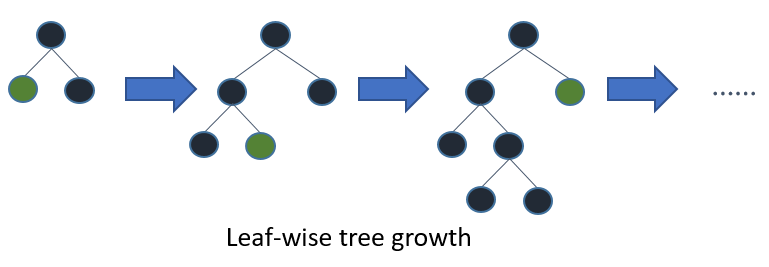
\includegraphics[width=0.35\textheight]{tesi_images/LGBM.png}
			\caption{LGBM: Leaf-wise tree growth}
			\label{fig:LGBM tree}
		\end{figure}
	
	\chapter{BDT: Electron and photon classification}	
		As said before, during the reconstruction not all the particles are easily reconstructed and therefore they are reconstructed both as electrons and photons. These particles are the 10\% of true electron and 30\% of true photon. 
		
		The analisys of these "ambiguous" particles is the last step in the discrimination process between electrons and photons. This analysis can be done in several ways. One of them is a classification algorithm with a gradient boosted decision tree (\textit{classification Supervised Learning}). In order to create a predictive model the GBDT is trained on single-particle samples of electrons and photons, with pile-up. For each true particle type there are two Pandas dataframes, one for reconstruction as an electron and the other for reconstruction as a photon. After the dataframes referring to the same type of true particle are merged, resulting in two dataframes: one for \textit{True Electron} and the other for \textit{True Photon}. After that these two dataframes are concatenated by tagging the double reconstructions from true electron with $truth=0$ and those from true photon with $truth=1$. Therefore the input particles are represented by $y_i$, which is 0 for true electron and 1 for true photon, and the score (model output) is $y_i^{pred} \epsilon [0,1]$.
		
		After removing the pile-up, the dataframe is splitted in the train (80\%) and the test (20\%) sets, using a Scikit Learn \cite{SKlearn} function. The train dataset is used to train the algorithm, whereas the test dataset is used as model input. If we did not do this split, we would introduce a bias.
		
		In order to explore as many cases as possible, three models have been created: all use the same discriminating variables, but they are trained on different portions of the training dataset.
		\begin{enumerate}
			\item a model generated by a GBDT trained on double reconstruction;
			\item a model generated by a GBDT trained on reconstruction flagged as “ambiguous” by the old ambiguity tool;
			\item a model generated by a GBDT trained on reconstruction flagged as “ambiguous” by the new ambiguity tool.
		\end{enumerate}
		
		Since at reconstruction level it is not possible to use a BDT and it is not possible to save the double reconstructions for each particle, due to the enormous memory cost it would involve, pre-classifiers (ambiguity tools) are used. To see the performance of these pre-classifiers, the models above are compared. The first is the ideal model, which has been trained as if there were infinite memory, and therefore is the theoretical limit. Therefore, the more models based on ambiguity tools approach the performance of the double reconstructions model, the better the applied preclassification is.
		
		\section{BDT training}
			Let's now focus on the BDT training
			\subsection{Discriminating features}
				In order to create a good model, the choice of the features it will have to work on is crucial. The most useful characteristics are those that present the greatest differences between photons and electrons, which are therefore more discriminating. It is also important to use features that guarantee the generality of the model. The features can be divided into two categories: electron and photon features.
				\subsubsection{Electron features}
					Electron features are those that characterize the particles reconstructed as electrons. Electrons have many hits in the first layers of detectors, as opposed to photons, because the most part of photons is still unconverted in the ID. So electron reconstructed as electrons (\texttt{true\_el/reco\_el}) should have more hits than photons reconstructed as electrons (\texttt{true\_ph/reco\_el}). This can be seen in the characteristics \texttt{el\_track\_hasInnermostHits} (a boolean, which says if the particle has hit the first expected layer or not), \texttt{el\_trkPixelHits} (a pixel hit counter), \texttt{el\_trkSiHits} (a silicon hit counter) shown in the figure \ref{fig:el_hit}.
					\begin{figure}[h!]
						\centering
						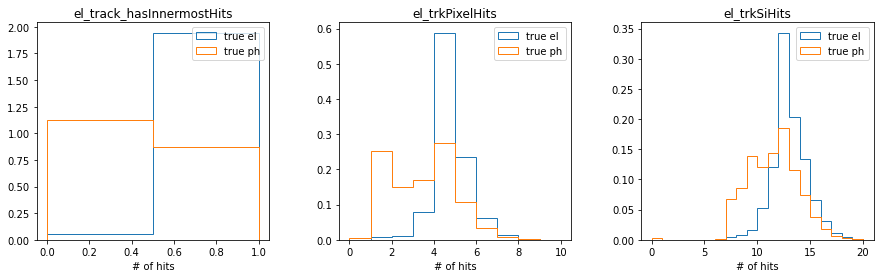
\includegraphics[width=0.7\textheight]{tesi_images/el_hit.png}
						\caption{}
						\label{fig:el_hit}
					\end{figure}
					
					The track quality, as it is determinated from the pixel and SCT hits, is different in the two cases as the physics quantities reconstructed from the track . This quantities are:
					\begin{itemize}
						\item \texttt{el\_track\_ep} is the ratio between the energy measured in the calorimeter and the moment $p_T$ measured in the ID. Photons tracks are worse than those of electrons and therefore they are not always matched with the right energy. So the Ep ratio could be far from 1 (Figure \ref{fig: ep}).
						\item \texttt{el\_trackz0} is the z coordinate, which runs along the detector, where the measurement of the reconstructed electron takes place (Figure \ref{fig: z0}).
						\item \texttt{el\_cl\_pt} is the cluster momentum $p_T$ of the reconstructed electron (Figure \ref{fig: pt}).
						\item \texttt{el\_cl\_eta} is the cluster $\eta$ of the reconstructed electron. Since photons convert more into the material we can see an increase of electrons reconstructed from real photons for $|\eta|>1.52$ (Figure \ref{fig: eta}).
					\end{itemize}
				
					\begin{figure}[ht]  
						\begin{minipage}[b]{0.5\linewidth}
							\centering
							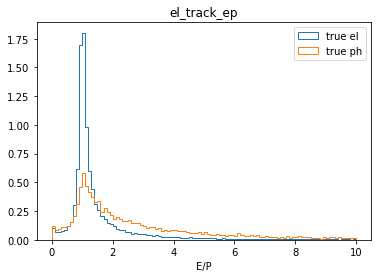
\includegraphics[width=.9\linewidth]{tesi_images/el_track_ep.png} 
							\caption{The \texttt{el\_track\_ep} distribution} 
							\label{fig: ep}
							\vspace{4ex}
						\end{minipage}%%
						\begin{minipage}[b]{0.5\linewidth}
							\centering
							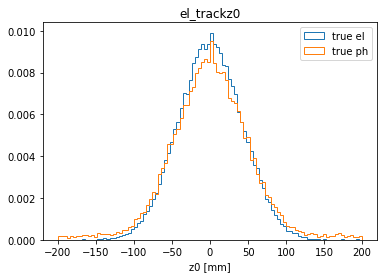
\includegraphics[width=.9\linewidth]{tesi_images/el_trackz0.png} 
							\caption{The \texttt{el\_trackz0} distribution}
							\label{fig: z0} 
							\vspace{4ex}
						\end{minipage} 
						\begin{minipage}[b]{0.5\linewidth}
							\centering
							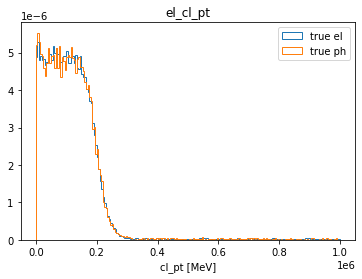
\includegraphics[width=.9\linewidth]{tesi_images/el_cl_pt.png} 
							\caption{The \texttt{el\_cl\_pt} distribution} 
							\label{fig: pt}
							\vspace{4ex}
						\end{minipage}%% 
						\begin{minipage}[b]{0.5\linewidth}
							\centering
							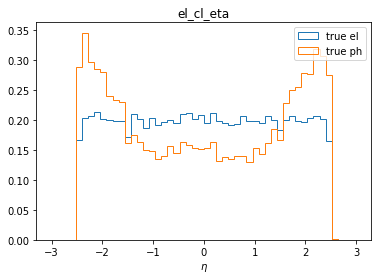
\includegraphics[width=.9\linewidth]{tesi_images/el_cl_eta.png} 
							\caption{The \texttt{el\_cl\_eta} distribution} 
							\label{fig: eta}
							\vspace{4ex}
						\end{minipage} 
					\end{figure}
				
				
				\subsubsection{Photon features}
					As electron, the photon quality track (of the pair $e^{+}e^{-}$) is discriminating and therefore also the Pixel/SCT hits and $p_t$.
					
					Other useful photon features for classification are those related to conversion:
					\begin{itemize}
						\item \texttt{ph\_zconv} (Fig. \ref{fig: zconv}) and \texttt{ph\_Rconv} (Fig. \ref{fig: Rconv}): these characteristics contain information of the conversion point in the coordinates R and z. \texttt{True\_el/reco\_ph} have a conversion point close to the point of interaction as their track starts from the beginning.
						
						\begin{figure}[h!]
							\begin{minipage}[b]{0.5\linewidth}
								\centering
								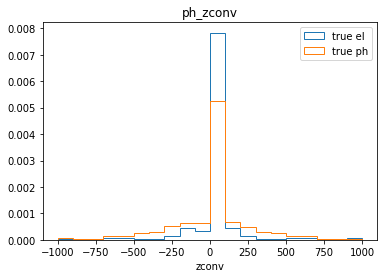
\includegraphics[width=.9\linewidth]{tesi_images/ph_zconv.png} 
								\caption{The \texttt{el\_track\_ep} distribution} 
								\label{fig: zconv}
								\vspace{4ex}
							\end{minipage}%%
							\begin{minipage}[b]{0.5\linewidth}
								\centering
								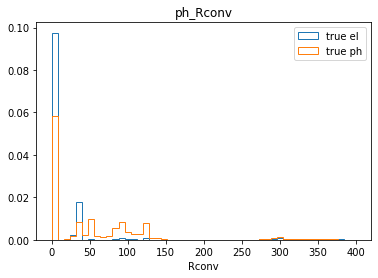
\includegraphics[width=.9\linewidth]{tesi_images/ph_Rconv.png} 
								\caption{The \texttt{el\_trackz0} distribution}
								\label{fig: Rconv} 
								\vspace{4ex}
							\end{minipage} 
						\end{figure}
						
						\item \texttt{ph\_pt1conv}, \texttt{ph\_pt2conv} and \texttt{ph\_ptconv} (Fig. \ref{fig: ph_pts}). All these three features have been scaled with \texttt{ph\_cl\_pt} to eliminate all kinematics information. 
						
						\begin{figure}[h!]	
							\centering
							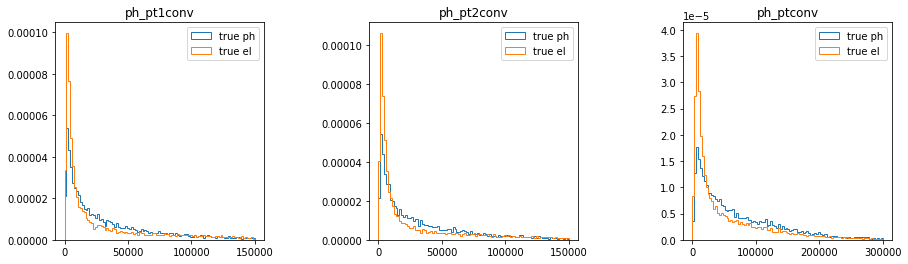
\includegraphics[width=1.\linewidth]{tesi_images/ph_pts.png} 
							\caption{The reconstructed photons momentum distributions} 
							\label{fig: ph_pts}
						\end{figure}
						
						\item \texttt{pt1conv/ptconv} contains information about conversion symmetry (Fig. \ref{fig: pt1_pt}). This characteristic for \texttt{true\_el/reco\_ph} tends to 1, since most of them have a single track. More information is presented in the Appendix \ref{Appex: sym}
						
						\begin{figure}[h!]	
							\centering
							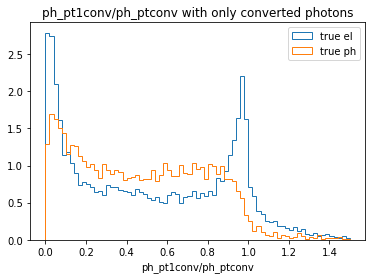
\includegraphics[width=.5\linewidth]{tesi_images/pt1_pt.png} 
							\caption{The reconstructed photons \texttt{pt1\_conv/pt\_conv} distributions} 
							\label{fig: pt1_pt}
						\end{figure}
					\end{itemize}
				
			\subsection{Parameters and Hyperparameter optimization}
				Parameters and hyperparameters regulate training and determine the performance of the model created. Hyperparameters are LGMB \cite{LGBM} adjustable parameters chosen for the training of a model, which regulate the training process. 
				
				The objective of the hyperparameter optimization is to search the various configurations of the hyperparameters, contained in the hyperparameter space, to find a configuration with the best performance. The hyperparameter space consists of two types of hyperparameters: discrete or continuous. Let's focus on the continuous ones, which are specified as a uniform distribution over a continuous range. 
				
				So after defining the space of the hyperparameters, we move on to the search for the best configuration. This search can be of various types:
				\begin{itemize}
					\item \textbf{random search}: in random search the hyperparameter values are randomly selected from the defined search space. It allows the  hyperparameter space to include both discrete and continuous hyperparameters;
					\item \textbf{grind search}: grid sampling performs a simple grid search on all possible values in the defined search space;
					\item \textbf{bayesian search}: bayesian sampling uses the knowledge of the previous samplings when choosing hyperparameter values, effectively attempting to improve the reported primary metric. The sample is selected based on the performance of the previous sample, so that the new sample improves the primary metric reported. 
				\end{itemize}
				The bayesian search is used by the Python library \textit{Hyperopt} \cite{Hyperopt}, which is implemented in the code in order to perform the optimization.
				
				The training parameters are listed in the Table \ref{tab:parameters} and the ones that have been optimized are:
				\begin{itemize}
					\item \textbf{bagging}: in bagging, several models of the same type are trained on different datasets (aggregation, typical of ensemble learning), each obtained from the initial dataset by random sampling with replacement (bootstrap).
					\item \textbf{number of leaves}: it is the maximum number of leaves, which a tree could have. It is useful to avoid overfitting.
					\item \textbf{feature fraction}: it is used when boosting is random forest. 0.82 feature fraction means LightGBM will used 82\% of parameters randomly in each iteration for building trees.
					\item \textbf{learning rate}: it determines the effect of each tree on the final outcome.
				\end{itemize}
				Before starting with the hyperparameter optimization the train dataset is splitted: 75\% stays as the train set whereas the 25\% becomes the validation set, which is used during the hyperparameter optimization training instead of the test set as validation. This is done with the aim of avoiding the introduction of a bias.
				
				After 200 searches the best hyperparameters are selected and used for the creation of the models, which have three different hyperparameters sets (shown in Table \ref{tab:parameters}).
				
				\begin{table}
					\centering
					\begin{tabular}{lccc}
						\toprule[1.5pt]
						\textbf{Parameter} & \textbf{Double Reco} & \textbf{Old ambiguous} & \textbf{New ambiguous} \\
						\midrule
						Metric & xentropy & xentropy & xentropy \\
						Objective & xentropy & xentropy & xentropy \\
						Bagging seed & 42  & 42 & 42 \\
						Feature fraction seed & 42 & 42 & 42 \\
						Is unbalance & True & True & True \\
						Number of leaves & 71 & 60 & 72 \\
						Feature fraction & 0.793 & 0.774 & 0.883 \\
						Bagging & 0.941 & 0.839 & 0.693 \\
						Learning rate & 0.026 & 0.032 & 0.025 \\
						\bottomrule[1.5pt]
					\end{tabular}
					\caption{Parameters and hyperparameters used in the models' training}
					\label{tab:parameters} 
				\end{table}
			
			\subsection{Training and Model}
				Once the hyperparameter optimisation is completed, algorithm training can begin. It is based on a LGBM function \texttt{lgb.train}, which has as input: parameter set, lgb train dataset, the maximum number of training steps, validation sets,  early stopping rounds. The validation sets are those on which the loss function is calculated during training. For training to create the model they must be \texttt{lgb\_train} and \texttt{lgb\_test}, whereas for the hyperparameters optimization training they are \texttt{lgb\_train} and \texttt{lgb\_valid}, as said before. \\
				To prevent overfitting, the model will train until the validation score stops improving. Validation score needs to improve at least every \texttt{early\_stopping\_rounds} round(s) to continue training \cite{LGBM}.
				
				Once the training is over, it is possible to analyse the model and how it uses the discriminatory variables. This is usually done through three plots:
				\begin{itemize}
					\item the Objective function plot. Its value is plotted after each iteraction for both the training and test set. This plot is uselful because a large difference between the train and test datasets may indicate overfitting (Fig \ref{fig:loss}).
					
					\begin{figure}[h!]
						\centering
						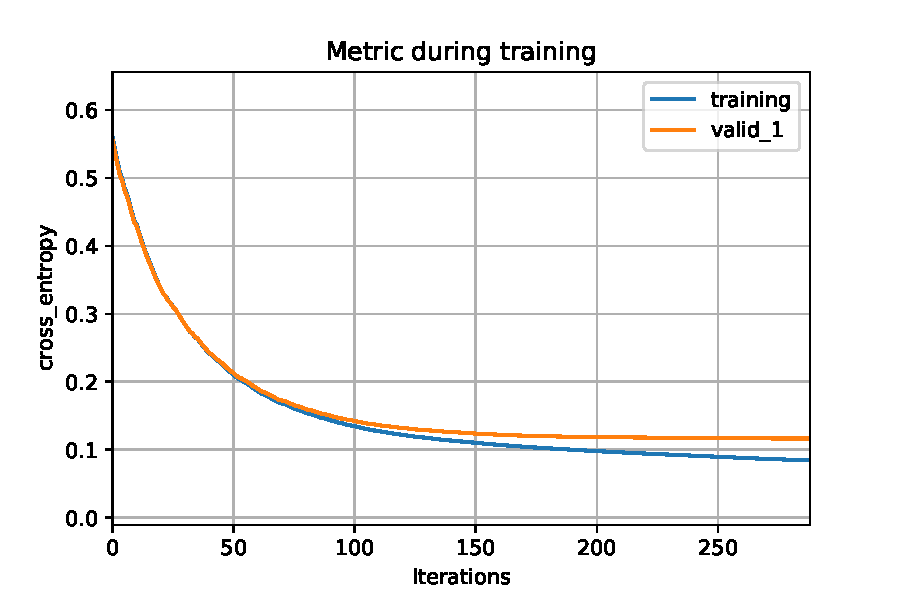
\includegraphics[width=.6\linewidth]{tesi_images/model_hyper_loss.pdf} 
						\caption{Loss value after each iteration, Model double reco}
						\label{fig:loss} 
					\end{figure}
					
					\item the feature importance plots. One shows the number of times that a feature was used in the splitting of a branch \ref{fig:importance}, the other the average training loss reduction gained when using a feature for splitting \ref{fig:gain}.
					
					\begin{figure}[h!]
						\centering
						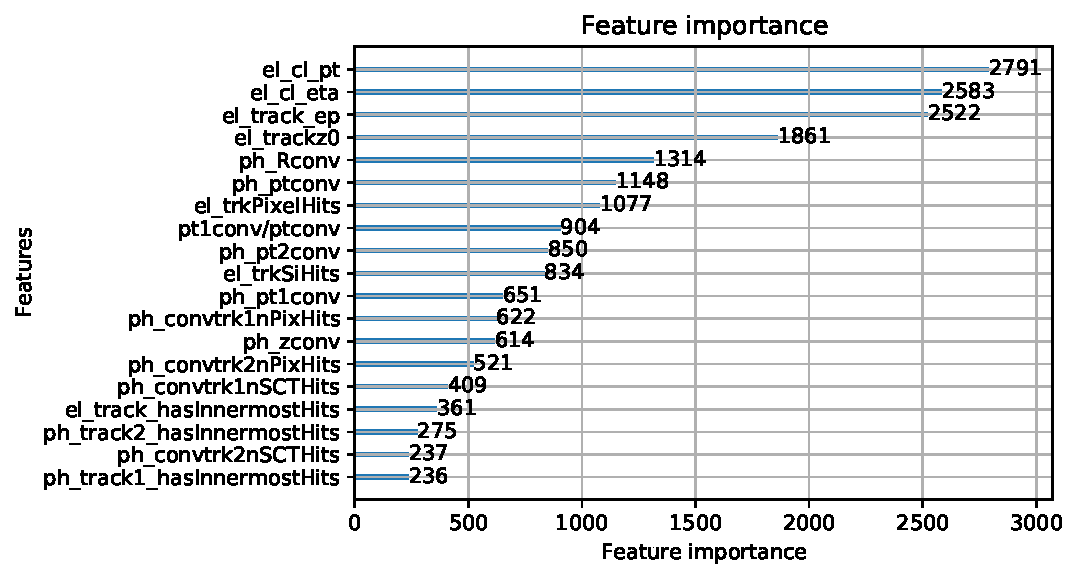
\includegraphics[width=.8\linewidth]{tesi_images/model_hyper_importance.pdf} 
						\caption{Feature importance, Model double reco}
						\label{fig:importance} 
					\end{figure}
				
					\begin{figure}[h!]
						\centering
						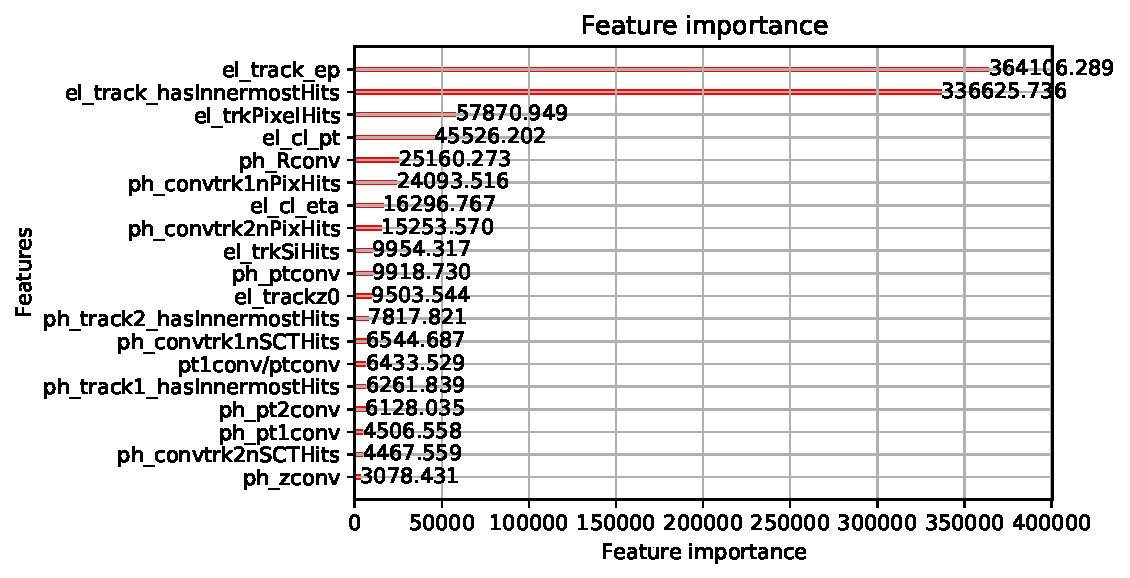
\includegraphics[width=.8\linewidth]{tesi_images/model_hyper_gain.pdf} 
						\caption{Feature importance Gain, Model double reco}
						\label{fig:gain} 
					\end{figure}
				\end{itemize}
			
		\section{BDT applied on test set}
			Once the models are created, these trained BDTs are applied to the test dataset. Each model gives to each particle a score between 0 and 1 according to its features. If the score is close to 0 the particle is classified mainly as electron, whereas if it tends to 1 as photon. 
			
			In order to evalute the models' efficiencies the scores, ROC and AUC are plotted and calculeted. The scores are plotted as two histograms, one for \textit{True Electrons} and the other for \textit{True Photons}, and compared,a shown in Figure \ref{fig:scores}.
		    \begin{figure}[h!]
		    	\centering
		    	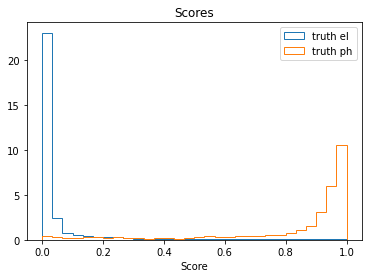
\includegraphics[width=.6\linewidth]{tesi_images/scores.png} 
		    	\caption{Scores histogram} 
		    	\label{fig:scores}
		    \end{figure}
		    
		    From these histograms is possible to extract the \textit{True Photons} efficiency, called True Positive Rate (TPR) 
			%$\epsilon_{ph}=$TPR$=\frac{\text{reco ph from trueph}}{\text{All ph}}$, 
			and the \textit{True Electron} efficiency, called False Positive Rate (FPR) 
			%$\epsilon_{el}=\frac{\text{reco el from true ph}}{\text{All el}}$ 
			by making cuts (thresholds) on the scoring range [0,1]. TPR, FPR and thresholds can also be obtained using a scikit-learn function \texttt{roc\_curve}, which has as input the $y^{true}$ and the model's predictions $y^{pred}$. 
			
			The ROC curve is a graph showing the performance of the  classification model at all thresholds. This curve plots two parameters: FPR versus TPR at different classification thresholds connecting the point (1,1) to (0,0). The perfomance estimator is the entire two-dimensional area underneath the entire ROC curve, called AUC, which is calculated using the scikit-learn function \texttt{auc(FPT,TPR)}. The closer the AUC is to 1, the more predictive the model is. 
			
		    Therefore, in order to calculate the performance of the various models they were applied to various portions of the test set by calculating the ROC curves and AUCs:
			\begin{itemize}
				\item double reconstructions model applied to double reconstructions (Fig \ref{fig:dr_dr}), old ambiguity tool ambiguous (Fig \ref{fig:dr_dr}) and new ambiguity tool ambiguous (Fig \ref{fig:dr_dr}) test sets.
				\item old ambiguous model applied to old ambiguity tool ambiguous (Fig \ref{fig:old_old}) test set.
				\item new ambiguous model applied to new ambiguity tool ambiguous (Fig \ref{fig:new_new}) test set.
				\item the previous examples with the single reco added to the test sets (Fig \ref{fig:all_roc}). To due they are applied on the same test set, they can be compared in one plot.
			\end{itemize}
			
			\begin{figure}[ht]  
				\begin{minipage}[b]{0.5\linewidth}
					\centering
					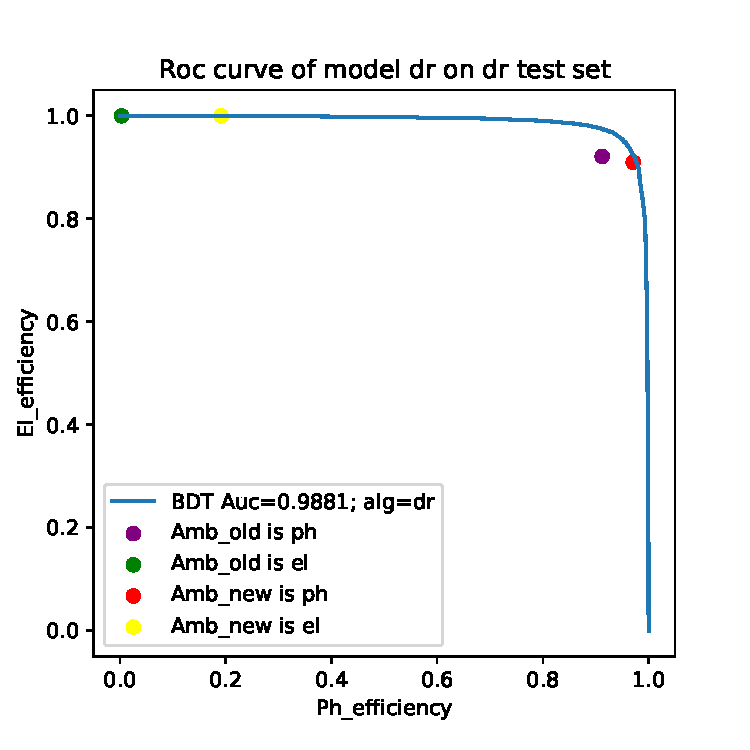
\includegraphics[width=1.\linewidth]{tesi_images/dr_dr.pdf}
					\caption{} 
					\label{fig:dr_dr}
					\vspace{4ex}
				\end{minipage}%%
				\begin{minipage}[b]{0.5\linewidth}
					\centering
					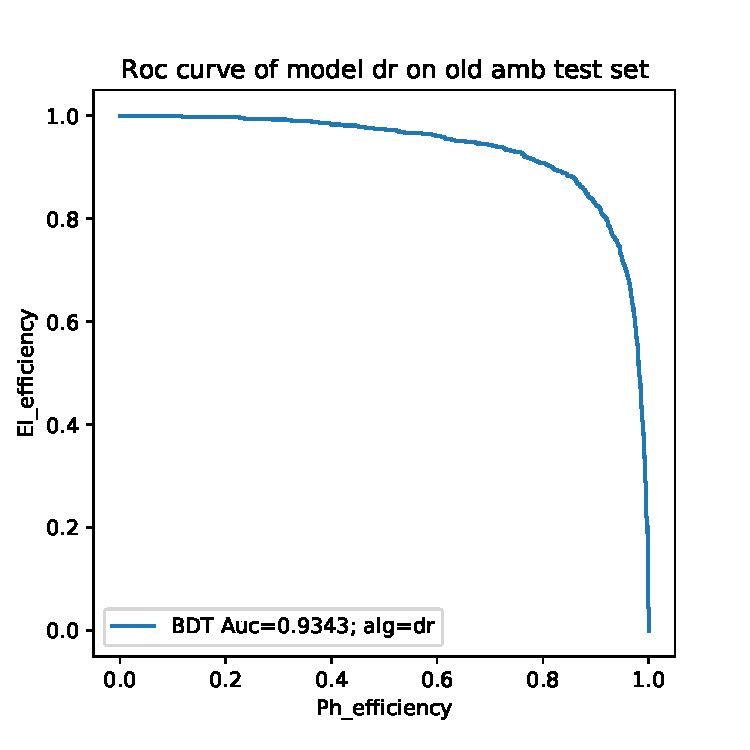
\includegraphics[width=1.\linewidth]{tesi_images/dr_old.pdf} 
					\caption{}
					\label{fig:dr_old} 
					\vspace{4ex}
				\end{minipage} 
				\begin{minipage}[b]{0.5\linewidth}
					\centering
					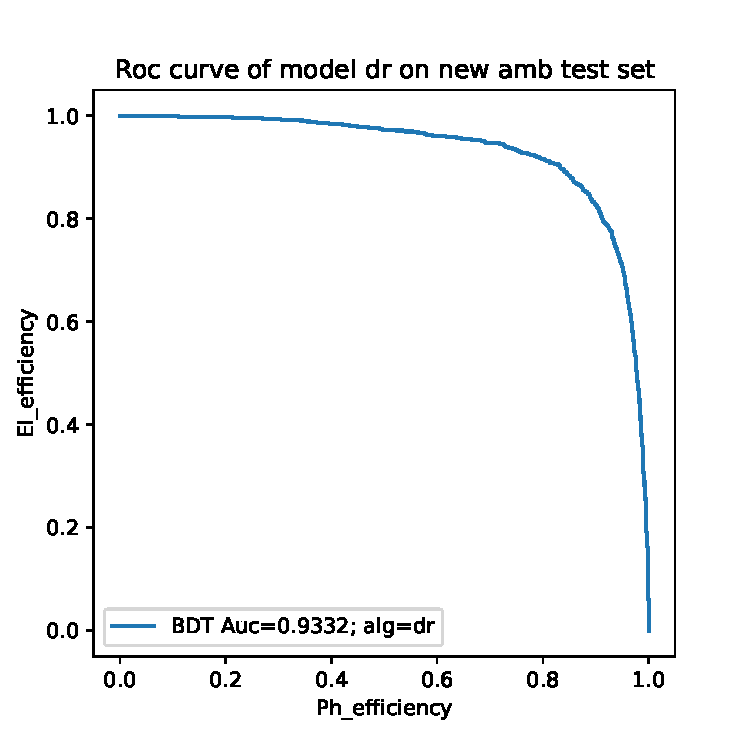
\includegraphics[width=1.\linewidth]{tesi_images/dr_new.pdf} 
					\caption{} 
					\label{fig:dr_new}
					\vspace{4ex}
				\end{minipage}%%
				\begin{minipage}[b]{0.5\linewidth}
					\centering
					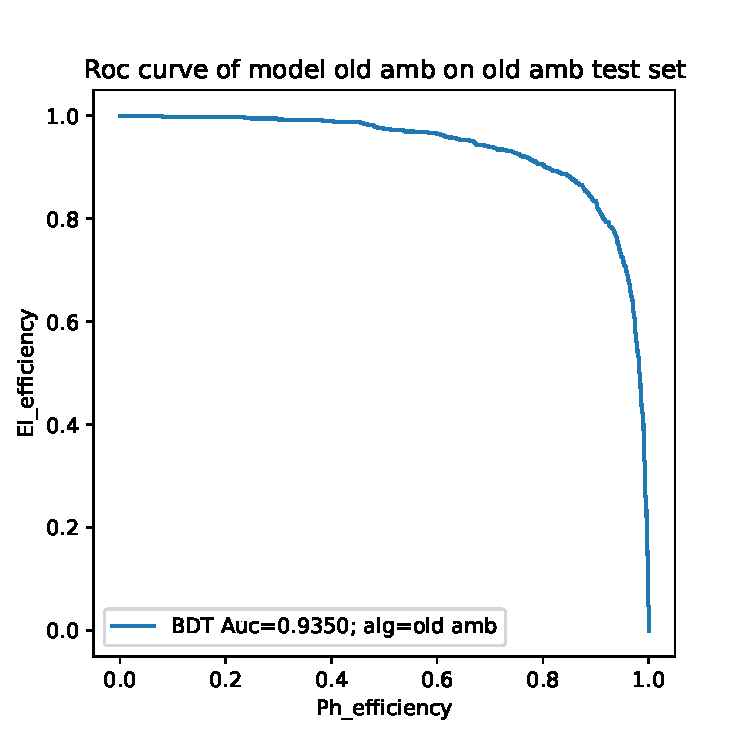
\includegraphics[width=1.\linewidth]{tesi_images/old_old.pdf} 
					\caption{} 
					\label{fig:old_old}
					\vspace{4ex}
				\end{minipage}
			\end{figure}
			\begin{figure}[ht]
				\begin{minipage}[b]{0.5\linewidth}
					\centering
					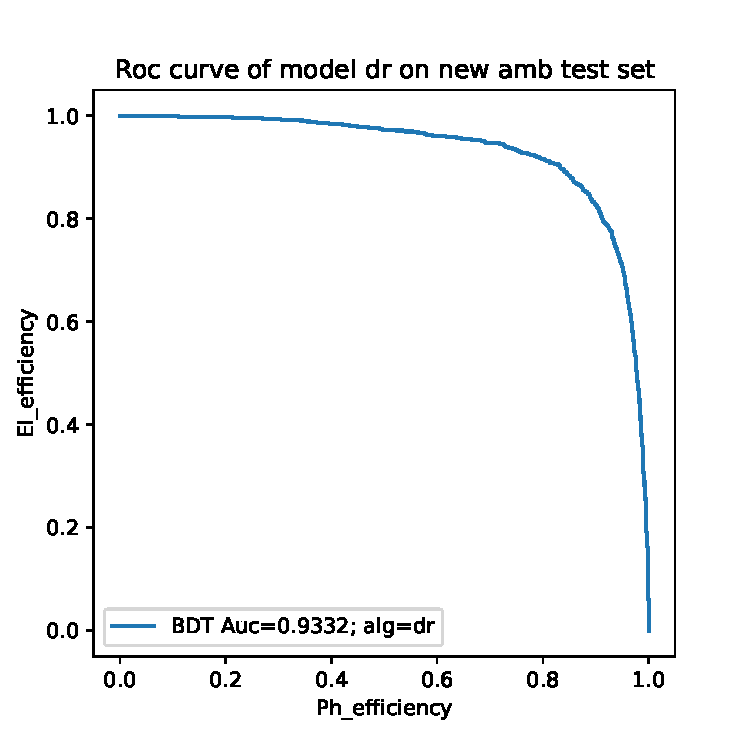
\includegraphics[width=1.\linewidth]{tesi_images/dr_new.pdf}
					\caption{} 
					\label{fig:new_new}
					\vspace{4ex}
				\end{minipage}%% 
				\begin{minipage}[b]{0.5\linewidth}
					\centering
					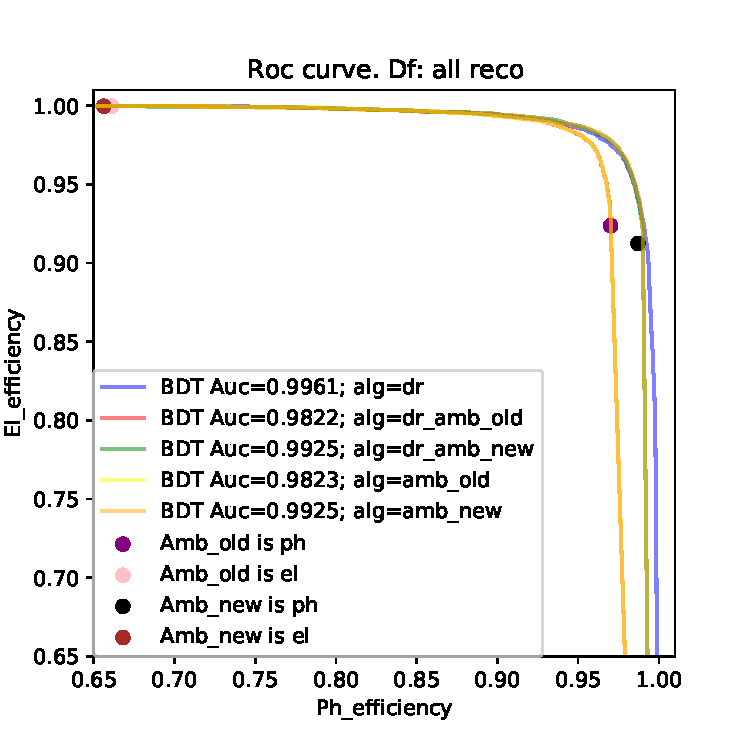
\includegraphics[width=1.\linewidth]{tesi_images/all_roc.pdf} 
					\caption{} 
					\label{fig:all_roc}
					\vspace{4ex}
				\end{minipage} 
			\end{figure}
		\section{BDT results}
			Questa sezione aspetto a scriverla per capire se devo aggiungere o meno i sample di fisica
		
	\chapter*{Conclusion}
		La conclusione aspetto a scriverla per capire se devo aggiungere o meno i sample di fisica
	\appendix
	\chapter{Conversion symmetry} \label{Appex: sym}
		Conversion symmetry plots of the reconstructed and converted photons. %We can see in Fig \ref{fig: pt1/2 el} and \ref{fig:pt12_ph}. that %\texttt{pt1/pt} and \texttt{pt2/pt} are anticorrelated.
		\begin{figure}[H]  
			\begin{minipage}[b]{0.5\linewidth}
				\centering
				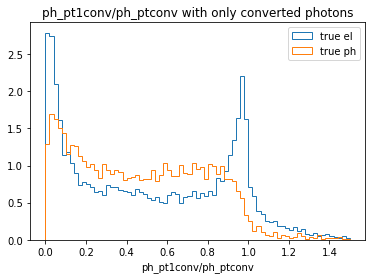
\includegraphics[width=.9\linewidth]{tesi_images/pt1_pt.png} 
				\caption{The \texttt{ph\_pt1conv/ph\_ptconv} distribution} 
				\label{fig: pt1/pt}
				\vspace{4ex}
			\end{minipage}%%
			\begin{minipage}[b]{0.5\linewidth}
				\centering
				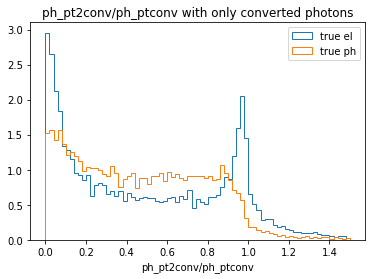
\includegraphics[width=.9\linewidth]{tesi_images/pt2_pt.png} 
				\caption{The \texttt{ph\_pt2conv/ph\_ptconv} distribution}
				\label{fig: pt2/pt} 
				\vspace{4ex}
			\end{minipage} 
			\begin{minipage}[b]{0.5\linewidth}
				\centering
				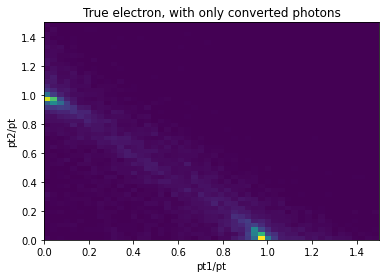
\includegraphics[width=.9\linewidth]{tesi_images/pt1_pt2_el_2D.png} 
				\caption{2D histogram of \texttt{pt1/pt} and \texttt{pt2/pt} distributions for \textit{True Electron}} 
				\label{fig: pt1/2 el}
				\vspace{4ex}
			\end{minipage}%% 
			\begin{minipage}[b]{0.5\linewidth}
				\centering
				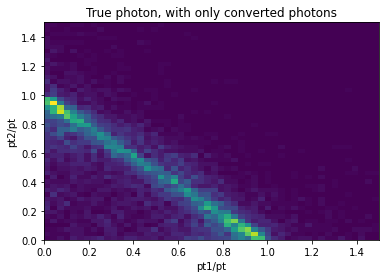
\includegraphics[width=.9\linewidth]{tesi_images/pt1_pt2_ph_2D.png} 
				\caption{2D histogram of \texttt{pt1/pt} and \texttt{pt2/pt} distributions for \textit{True Photon}} 
				\label{fig:pt12_ph}
				\vspace{4ex}
			\end{minipage} 
		\end{figure}
		
	\clearpage		
	\begin{thebibliography}{32}
			
			%%%%%%%%%%%%%%%%%%%%%%%%%%%%%%%%%%%%%%%%%%%%%%%%%%%%%%%%%%%%%%%%%%%%%%%%%%%%%%%%%%%%%%%%%%%%%%%%%%%%%%%%%%%%%%%%%%%%%%%%%%%%%%%%%%%%%%%%%%%%%%%%%%%%%%%%%%%%%%%%%%%%%%%%%%%%%%%%%%%%%%%%%%%%%%%%%%%%%%%%%%%%%%
			%\textbf{\Large Chapter 2} 
			
			% 1 %
			\bibitem{LHC design} European organization for nuclear research, \textit{LHC design report}, CERN libraries, Geneva (2004). \url{http://cds.cern.ch/record/782076/files/}
			% 2 %
			\bibitem{LHC introduction} F. Gianotti, \textit{Collider physics: LHC}, EP Division, CERN, Geneva, Switzerland. \url{https://cds.cern.ch/record/458489/files/p219.pdf}
			% 3 %
			\bibitem{LHC site}
			\textit{The Large Hadron Collider (LHC)}
			\url{https://home.cern/science/accelerators/large-hadron-collider}
			% 4 % 
			\bibitem{Acc. complex} \url{https://cds.cern.ch/record/2255762/files/CERN-Brochure-2017-002-Eng.pdf}
			% 5 %
			\bibitem{ATLAS intro} \url{https://home.cern/science/experiments/atlas}
			% 6 % 
			\bibitem{ATLAS config}  The ATLAS Collaboration et al 2008 JINST3 S08003
			\url{https://iopscience.iop.org/article/10.1088/1748-0221/3/08/S08003/pdf}
			% 7 %
			\bibitem{ATLAS TDR}
			\textit{Technical Design Report:  A High-Granularity Timing Detector for the ATLAS Phase-II Upgrade}, ATLAS Collaboration, CERN, CERN-LHCC-2020-007. ATLAS-TDR-031, Geneva, Jun 2020
			\url{https://cds.cern.ch/record/2719855}
			% 8 % 
			\bibitem{Inner Detector} H. Pernegger, \textit{The Pixel Detector of the ATLAS Experiment for LHC Run-2}, ATL-INDET-PROC-2015-001. \url{https://cds.cern.ch/record/1985432/files/ATL-INDET-PROC-2015-001.pdf}
			% 9 %
			\bibitem{SCT} J.R. Pater \textit{The ATLAS SemiConductor Tracker operation and performance}, 2012 JINST7 C04001. \url{https://iopscience.iop.org/article/10.1088/1748-0221/7/04/C04001/pdf}
			% 10 % 
			\bibitem{TRT} Adrian Vogel \textit{ATLAS Transition Radiation Tracker (TRT): Straw Tube Gaseous Detectors at High Rates}, CERN,
			Geneva, ATL-INDET-PROC-2013-005, Apr 2013, ATL-INDET-PROC-2013-005. \url{https://cds.cern.ch/record/1537991}
			% 11 %
			\bibitem{Calorimetry}
			\url{http://ific.uv.es/~cabrera/teaching/atlas_i.pdf}\\
			% 12 %
			\bibitem{Calo intro}
			\url{https://atlas.cern/discover/detector/calorimeter}
			% 13 %
			\bibitem{Muon system}
			\textit{The ATLAS muon spectrometer: calibration and pattern recognition}, N. Van Eldik, CERN-THESIS-2007-045, 2007,
			\url{http://cds.cern.ch/record/1044839}
			% 14 %
			\bibitem{Trigger intro}
			\textit{Trigger and Data Acquisition System}
			\url{https://atlas.cern/discover/detector/trigger-daq}	
			% 15 % 
			\bibitem{Trigger system}
			\textit{The Run-2 ATLAS Trigger System: Design, Performance and
			Plan}, Martin zur Nedden, CERN, ATLAS Collaboration, Geneva, Dec 2016, ATL-DAQ-PROC-2016-039,
			\url{https://cds.cern.ch/record/2238679}
			% 16 % 
			\bibitem{STD Model}
			\textit{The ATLAS Physics}
			\url{https://atlas.cern/discover/physics}
			% 17 %
			\bibitem{CMS} 
			\textit{The CMS experiment at the CERN LHC}, The CMS Collaboration
			\url{https://doi.org/10.1088%2F1748-0221%2F3%2F08%2Fs08004}
			% 18 %
			\bibitem{Higgs}
			\textit{Observation of a new particle in the search for the Standard Model Higgs boson with the ATLAS detector at the LHC},
			The ATLAS Collaboration, In: \textit{Phys. Lett. B} 716.arXiv:1207.7214.CERN-PH-EP-2012-218 (Aug. 2012) DOI:\url{https://doi.org/10.1016/j.physletb.2012.08.020}, URL:\url{http://www.sciencedirect.com/science/article/pii/S037026931200857X}
			%%%%%%%%%%%%%%%%%%%%%%%%%%%%%%%%%%%%%%%%%%%%%%%%%%%%%%%%%%%%%%%%%%%%%%%%%%%%%%%%%%%%%%%%%%%%%%%%%%%%%%%%%%%%%%%%%%%%%%%%%%%%%%%%%%%%%%%%%%%%%%%%%%%%%%%%%%%%%%%%%%%%%%%%%%%%%%%%%%%%%%%%%%%%%%%%%%%%%%%%%%%%%%%
		 	%\textbf{\Large Chapter 2} 
		 	
			% 10 %
			\bibitem{El ph intro} Wu Xin, Clark Allan and Campanelli Mario \textit{Electron and photon identification in ATLAS}, Springer Berlin Heidelberg, Berlin, Heidelberg, 2006
			\url{https://link.springer.com/chapter/10.1007/978-3-540-32841-4_21} 
			% 11 %
			\bibitem{El ph reco}
			\textit{Electron and photon performance measurements with the {ATLAS} detector using the 2015-2017 {LHC} proton-proton collision data}
			\url{https://iopscience.iop.org/article/10.1088/1748-0221/14/12/P12006}
			% 12 %
			\bibitem{In-out alg} \textit{A neural network clustering algorithm for the ATLAS silicon pixel detector}, The ATLAS collaboration
			\url{{https://doi.org/10.1088%2F1748-0221%2F9%2F09%2Fp09009}}
			% 13 % 
			\bibitem{Track reco}
			\url{https://link.springer.com/content/pdf/10.1140/epjc/s10052-019-7140-6.pdf}in
			% 14 % 
			\bibitem{ID reco alg} \textit{Optimisation of the ATLAS Track Reconstruction Software for Run-2}, Andreas Salzburger, CERN, Switzerland, \url{http://iopscience.iop.org/1742-6596/664/7/072042}
			% 15 % 
			\bibitem{Identification} \textit{Electron and photon identification with the ATLAS detector}, Proklova Nadezda, ATLAS Collaboration, Aug 2018, ATL-PHYS-SLIDE-2018-606, \url{http://cds.cern.ch/record/2634679}
			% 16 %
			\bibitem{El ph isol} \textit{Search for supersymmetry with a compressed mass spectrum using the ATLAS detector}, Rossini Lorenzo, \url{http://hdl.handle.net/2434/683343 }\\
			%%%%%%%%%%%%%%%%%%%%%%%%%%%%%%%%%%%%%%%%%%%%%%%%%%%%%%%%%%%%%%%%%%%%%%%%%%%%%%%%%%%%%%%%%%%%%%%%%%%%%%%%%%%%%%%%%%%%%%%%%%%%%%%%%%%%%%%%%%%%%%%%%%%%%%%%%%%%%%%%%%%%%%%%%%%%%%%%%%%%%%%%%%%%%%%%%%%%%%%%%%%%%%%
			%\textbf{\Large Chapter 3}
			% 17 %
			\bibitem{Lifelong ML} \textit{Lifelong Machine Learning}, Zhiyuan Chen and Bing Liu, Morgan \& Claypool Publishers, Nov 2016, \url{https://www.cs.uic.edu/~liub/lifelong-machine-learning-draft.pdf}
			% 18 %
			\bibitem{ML categories} \textit{Machine Learning: A Probabilistic Perspective}, Kevin P. Murphy, The MIT Press, \url{https://scholar.google.it/scholar?q=K.P.+Murphy,+Machine+Learning.+A+Probabilistic+Perspective+,+MITpress+(2012)&hl=it&as_sdt=0&as_vis=1&oi=scholart}
			% 19 % 
			\bibitem{GBT} \url{https://xgboost.readthedocs.io/en/latest/tutorials/model.html}
			% 20 %
			\bibitem{Decision Tree} \textit{4Classification:Basic Concepts,Decision Trees, andModel Evaluation}, \url{https://www-users.cs.umn.edu/~kumar001/dmbook/ch4.pdf}
			% 20 % 
			\bibitem{LGBM} \textit{LightGBM’s documentation} 
			\url{https://lightgbm.readthedocs.io/en/latest/}
			
			%%%%%%%%%%%%%%%%%%%%%%%%%%%%%%%%%%%%%%%%%%%%%%%%%%%%%%%%%%%%%%%%%%%%%%%%%%%%%%%%%%%%%%%%%%%%%%%%%%%%%%%%%%%%%%%%%%%%%%%%%%%%%%%%%%%%%%%%%%%%%%%%%%%%%%%%%%%%%%%%%%%%%%%%%%%%%%%%%%%%%%%%%%%%%%%%%%%%%%%%%%%%%%%
			%\textbf{\Large Chapter 4}
			
			% 33 %
			\bibitem{SKlearn}
			\textit{Scikit-learn: Machine Learning in Python}, Pedregosa et al., JMLR 12, pp. 2825-2830, 2011.
			% 34 %
			\bibitem{Hyperopt}
			\textit{Making a Science of Model Search: Hyperparameter Optimization in Hundreds of Dimensions for Vision Architectures. To appear in Proc. of the 30th International Conference on Machine Learning}, J. Bergstra, D. Yamins, D. D. Cox, ICML, 2013
			
	\end{thebibliography}
\end{document}